\documentclass[12pt]{article}

% Figures
\usepackage{graphicx}
\usepackage[list=true]{subcaption}
\graphicspath{{../../plots/}{../../tikz/}{../../img/}}
\usepackage[section]{placeins} % require floats to appear in the section they are defined

% fonts and appearance
\usepackage{amsmath, amsfonts, physics, siunitx, nicefrac}
\usepackage[american]{babel} 
\usepackage[T1]{fontenc} % improved font encoding
\usepackage[ttscale=0.8]{libertine}
\usepackage{fontawesome5}
\usepackage[format=plain, textfont=it]{caption}

% page size and margins
\usepackage{geometry}
\geometry{letterpaper,top=1in, bottom=1in, left=1in, right=2in}

% footer
\usepackage{fancyhdr}
\usepackage{lastpage}
\usepackage[en-US]{datetime2}
\fancyhf{}
\fancyhead[L]{CONFIDENTIAL DRAFT by J. Doss-Gollin \& K. Keller}
\fancyhead[R]{\DTMnow}
\fancyfoot[R]{page~\thepage~of~\pageref{LastPage}}
\pagestyle{fancy}

% TO DO NOTES
\usepackage{xcolor} % list of colors at https://en.wikibooks.org/wiki/LaTeX/Colors
\definecolor{giallo}{HTML}{F0BC42} % https://teamcolorcodes.com/a-s-roma-color-codes/
\definecolor{rosso}{HTML}{8E1F2F}
\definecolor{grigio}{HTML}{CACACC}
\definecolor{nero}{HTML}{000000}
\usepackage[textsize=scriptsize]{todonotes}
\setlength{\marginparwidth}{1.5in}
\newcommand{\james}[1]{\todo[color=giallo, textcolor=nero]{\textbf{ATTN James:~}#1}} % if desired create a custom command for each author
\newcommand{\klaus}[1]{\todo[color=rosso, textcolor=grigio]{\textbf{ATTN Klaus:~}#1}}

% better tables
\usepackage{booktabs}
\usepackage{array}
\newcommand{\PreserveBackslash}[1]{\let\temp=\\#1\let\\=\temp}
\newcolumntype{C}[1]{>{\PreserveBackslash\centering}p{#1}}
\newcolumntype{R}[1]{>{\PreserveBackslash\raggedleft}p{#1}}
\newcolumntype{L}[1]{>{\PreserveBackslash\raggedright}p{#1}}

% better lists
\usepackage[inline]{enumitem}
\setlist{nosep}

% authors
\usepackage{authblk}
\title{Mainstreaming Climate Adaptation Requires Subjective Integration of Deep Uncertainties}
\author[1]{James Doss-Gollin}
\author[2]{Klaus Keller}
\affil[1]{Department of Civil and Environmental Engineering, Rice University}
\affil[2]{Thayer School of Engineering, Dartmouth College}
\renewcommand*{\Affilfont}{\normalsize\normalfont}

% ACRONYMS
\usepackage[acronym,nopostdot,nonumberlist,shortcuts,]{glossaries}
\newacronym{bdt}{BDT}{Bayesian decision theory}
\newacronym{bfe}{BFE}{base flood elevation}
\newacronym[]{cdf}{CDF}{cumulative distribution function}
\newacronym{fema}{FEMA}{the Federal Emergency Management Agency}
\newacronym{gcm}{GCM}{general circulation model}
\newacronym[]{gev}{GEV}{generalized extreme value}
\newacronym{iid}{IID}{independent and identically distributed}
\newacronym{ipcc}{IPCC}{International Panel on Climate Change}
\newacronym{lsl}{LSL}{local mean sea level}
\newacronym{mcmc}{MCMC}{Markov Chain Monte Carlo}
\newacronym{pdf}{PDF}{probability density function}
\newacronym{rcp}{RCP}{representative concentration pathway}
\newacronym{msl}{MSL}{mean relative sea level}
\newacronym{rdm}{RDM}{robust decision making}
\newacronym[plural=SOWs,descriptionplural=states of the world]{sow}{SOW}{state of the world}
\newacronym{tc}{TC}{tropical cyclone}

\usepackage{xspace}
\makeatletter
\DeclareRobustCommand\onedot{\futurelet\@let@token\@onedot}
\def\@onedot{\ifx\@let@token.\else.\null\fi\xspace}
\def\eg{\emph{e.g}\onedot} \def\Eg{\emph{E.g}\onedot}
\def\ie{\emph{i.e}\onedot} \def\Ie{\emph{I.e}\onedot}
\def\etc{\emph{etc}\onedot} \def\vs{\emph{vs}\onedot}

\usepackage{xspace}
\makeatletter
\DeclareRobustCommand\onedot{\futurelet\@let@token\@onedot}
\def\@onedot{\ifx\@let@token.\else.\null\fi\xspace}
\newcommand{\usd}[1]{\SI{#1}[\$]{}}
\def\eg{\emph{e.g}\onedot} \def\Eg{\emph{E.g}\onedot}
\def\ie{\emph{i.e}\onedot} \def\Ie{\emph{I.e}\onedot}
\def\etc{\emph{etc}\onedot} \def\vs{\emph{vs}\onedot}

% use biblatex
\usepackage{csquotes}
\usepackage[
  backend=biber,
  doi=true,
  url=false,
  isbn=false,
  style=authoryear-comp,
  natbib=true,
  backref=false,
  maxbibnames=10,
  maxcitenames=2,
  uniquename=false,
  uniquelist=false,
  sorting=nyt,
  giveninits=true,
]{biblatex}
\renewbibmacro{in:}{}
\AtEveryBibitem{\clearfield{month}\clearfield{day}\clearfield{pages}\clearlist{language}}
\addbibresource{library.bib}

% load this last
\usepackage[hidelinks]{hyperref}
\usepackage{cleveref}

% up to 1250 words
\begin{document}
\maketitle
\thispagestyle{empty}

\begin{abstract}
    National agencies, regional governments, and individual households manage flood risk through a combination of standards and cost-benefit analyses that rely on estimates of flood hazard.
    One example is house elevation: \acrlong{fema} recommends a house located in the floodplain be elevated to the \acrlong{bfe} (typically the 100 year flood level) plus a freeboard (typically \SI{1}{ft}) if doing so would pass a cost-benefit test.
    Under stationarity, the probabilities used for this analysis (\ie to estimate the 100 year flood height or to perform the cost-benefit analysis) can be estimated using empirical frequencies from the observational record.
    However, growing recognition of nonstationarity motivates a forward-looking approach.
    Efforts to incorporate nonstationarity hazard into planning have struggled to overcome deep uncertainties in projections of future hazard because different models  may fit the observed data equally well but yield very different estimates of future hazard, and there is often no objective way to choose between them (\ie, equifinality).
    In this paper we use a didactic case study of deciding if and how high to elevate a single house in the coastal zone to illustrate a decision theoretic framework that combines exploratory modeling, robust decision making, and subjective Bayesian philosophy.
    We first use exploratory modeling to illustrate that there is no dominant strategy; instead, there are instrinsic tradeoffs between performance under low- and high-sea level rise scenarios.
    Next, we map the tradeoff between up-front cost and expected damages for each of sixteen models of future sea level rise to illustrate that the choice of which model to use has a strong influence on estimated trade-offs, cost-benefit analyses, or policy prescriptions.
    To overcome these shortcomings, we propose and illustrate a computationally efficient method for scenario weighting conditional on a subjective prior belief over future sea level rise.
    This method provides a transparent framework for synthesizing deep uncertainties, facilitating critique and dialogue around necessarily subjective decisions.
    It can be applied beyond nontationary flood risk management to other problems in climate adaptation, calculating the social cost of carbon, and more.
\end{abstract}

Key points
\begin{enumerate}
    \item
\end{enumerate}

\clearpage
\section{Introduction}\label{sec:introduction}

Estimates of flood hazard affect peoples' lives
\begin{enumerate}
    \item Floods affect lots of people and property
    \item Climate change and exposure making floods worse
    \item Floodplain management: $T$ year flood
    \item Some cost-benefit analysis and lots of design standards / heuristics
\end{enumerate}
One example is floodproofing
\begin{enumerate}
    \item Literature on floodproofing and building-scale vulnerability reduction measures
    \item This works great!
    \item But who should use it? We're still using standards.
    \item Prior studies have found that floodproofing and building-scale vulnerability reduction measures, including house elevation, can effectively reduce local flood damages in many contexts \citep{demoel_reducing:2014,deruig_building:2020,kreibich_building:2005,slotter_floodproofing:2020,Rozer:2016dn,mobley_mitigation:2020,aerts_cost:2018}.
          Official guidance for homeowners, notably from \gls{fema}, recommends elevating to the \gls{bfe} (typically the \SI{100}{year} flood) plus a freeboard \citep{fema_retrofitting:2014,asce_24-14:2015,fema_retrofitting:2014} but recent suggests scope for improvement.
          For example, \citet{xian_elevation:2017} used a cost-benefit analysis to demonstrate that tailoring recommendations to the inital elevation of a structure can reduce expected costs.
          \citet{zarekarizi_suboptimal:2020} show that neglecting uncertainty in discount rate, house lifespan, flood risk, and depth-damage curves can lead to maladaptation.
          Yet these studies are silent on the question of how nonstationary flood hazard should factor into this decision.
\end{enumerate}
Nonstationarity
\begin{enumerate}
    \item These analyses all rely on \glspl{pdf}
    \item Growing evidence for nonstationarity in a wide variety of hydroclimate processes
    \item We often focus on climate change as a driver but sometimes local modifications matter just as much \citep{Merz:2014gf}
    \item Even where risk-based analyses are used, this problem recommendations
    \item Yet stationarity remains the dominant assumption because it is immortal \citep{Montanari:2014hl} or undead \citep{Serinaldi:2015bq}
    \item Bonstationarity of flood hazard is already evident in many places, especially in coastal areas where \gls{msl} is clear.
    \item On the other, efforts to find objective methods for quantifying nonstationarity, eg of precipitation \citep{atlas14_texas:2018} or flood frequency \citep{bulletin17c:2019}, have struggled to find a satisfactory approach because factors like future emissions and localized climate response create deep uncertainties that resist objective quantification
\end{enumerate}
It matters how you prepare
\begin{enumerate}
    \item Equifinality problem: different models diverge even if they fit the historical record well
    \item Over- and under-design can each be costly \citep{DossGollin:2019}
    \item On the one hand, overly optimistic assumptions of future risk can lead to unacceptably high risk of failure in the future if additional investments are not made.
          For example, a failure to prepare Texas's interconnected natural gas, electricity, and water systems for temperatures that had been observed in the past 30 years caused cascading failures with disparate impacts \citep{doss-gollin_txtreme:2021,busby_cascadingrisks:2021}.
    \item On the other, unless opportunity costs are negligible, designing for a too-pessimistic scenario can contribute to maladptation by limiting resource availability in the future. For example,\ldots\ldots\james{add an example of a maladaptive megaproject -- look to sustainability science or the arguments in \citet{ansar_bigisfragile:2017}, something by Flyvbjerg, \etc}
\end{enumerate}
A quick philosophical literature review of how people have approached and interpreted this problem
\begin{enumerate}
    \item This motivates subjective approaches for designing for nonstationarity.
    \item There's a little bit of RDM-style work on floods \citep{sriver_sealevel:2018,garner_slrise:2018,lempert_slr:2012}
    \item Model choice in $\mathcal{M}$-open case
    \item Philosophy of Bayesian statistics and decision making -- explain subjective probability
\end{enumerate}
Case study
\begin{enumerate}
    \item House elevation in the coastal zone as a specific example of a problem where both over- or under-investment could be a problem
    \item Federal guidance uses both standards (floodplain, \gls{bfe}) and cost-benefit analysis (does it pass test?)
    \item Be sure to note that this has parallels to lots of other engineering design guidance.
    \item \citet{xian_elevation:2017}: one size does not fit all
    \item \citet{zarekarizi_suboptimal:2020}: neglecting uncertainty leads to bad outcomes
\end{enumerate}
Plan d'attaque
\begin{enumerate}
    \item Research questions
          \begin{description}
              \item[Q1] What are the potential benefits to homeowners of changing threshold-based guidance to risk-based guidance under nonstationary flood hazard?
              \item[Q2] How does risk-based guidance change under different assumptions of physical model structure and human emissions forcings?
              \item[Q3] How can deep uncertainties be transparently and consistently synthesized for decision analysis?
          \end{description}
    \item In \cref{sec:case-study} we describe our case study in Norfolk, VA.
    \item  in \cref{sec:multiple-simulation} we analyze each simulation (\ie, realizations from these \glspl{pdf}) independently and illustrate .
    \item  in \cref{sec:multiple-pdf} we consider the design problem as a set of ``multiple \glspl{pdf}'' and use these findings to motivate theoretical advances.
    \item  in \cref{sec:synthesizing} we present a probabilistic method for synthesizing simulations from multiple \glspl{pdf} and illustrate the advantages and potential pitfalls of this approach.
    \item  in \cref{sec:conclusions} we briefly summarize our findings, discuss implications for engineering practice, and identify  future research needs.
\end{enumerate}


\section{Case study}\label{sec:case-study}

We model a single, one-time decision of whether to elevate a house, and if so by how much (\cref{fig:xlrm}), for a \emph{hypothetical} house in Norfolk, VA.
For interpretability, we focus on deep uncertainty in \gls{msl} and treat other model parameters as fixed quantities or as outputs from a single probabilsitic model, as shown in \cref{tab:uncertainties}.
We evaluate this decision for each of many possible simulations of \gls{msl} using a combined engineering-economic model based on that of \citet{zarekarizi_suboptimal:2020}.
In the remainder of this section we discuss data sources and models.

\begin{table}
    \centering
    \caption{
        Summary of parameters, their notation, and how their uncertainty is modeled.
    }\label{tab:uncertainties}
    \begin{tabular}{l l p{3in} l}
        \toprule
        Name             & Symbol            & Uncertainty                                                                          & See more                     \\
        \midrule
        \Gls{msl}        & $\overline{y}(t)$ & Deeply uncertain: four physical models $\times$ four \acrshort{rcp} scenarios        & \cref{sec:sea-level}         \\
        Storm surge      & $y'(t)$           & Probabilistic: Bayesian inference on a stationary \acrshort{gev} model               & \cref{sec:storm-surge}       \\
        Ann-max flood    & $y(t)$            & Deterministic: $y(t)=\overline{y}(t)+y'(t)$                                          &                              \\
        Discount rate    & $1-\gamma$        & Fixed at 3\%                                                                         & \cref{sec:led}               \\
        Depth-damage     & $D(h-y)$          & Deterministic: based on HAZUS model                                                  & \cref{fig:cost-depth-damage} \\
        Elevation cost   & $C(\Delta h)$     & Deterministic: a piecewise linear model following \citet{zarekarizi_suboptimal:2020} & \cref{fig:cost-up-front}     \\
        Initial height   & $h_0$             & Deterministic: \SI{1}{ft} below the \gls{bfe} unless otherwise noted                 &                              \\
        House floor area &                   & Deterministic: \SI{1500}{ft^2} unless otherwise noted                                &                              \\
        Structural value &                   & Deterministic: \usd{200000} unless otherwise noted                                   &                              \\
        House lifetime   &                   & Deterministic: 70 years unless otherwise noted                                       &                              \\
        \bottomrule
    \end{tabular}
\end{table}

\begin{figure}
    \centering
    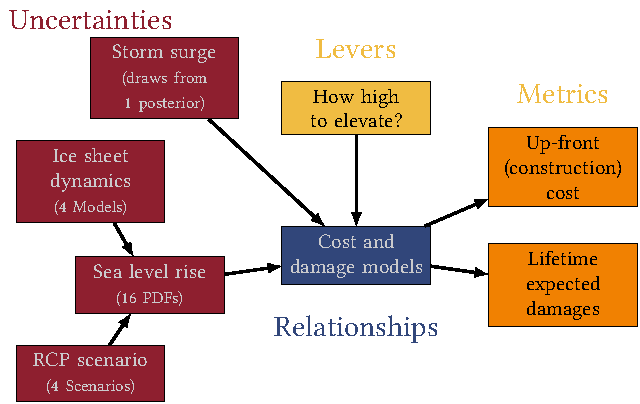
\includegraphics[width=4in]{xlrm.pdf}
    \caption{
        Conceptual diagram of the decision problem.
        A \gls{sow} consists of a description of the uncertain factors (red).
        We model a single decision (yellow).
        For each combination of \gls{sow} and policy, the system model (blue) is used to calculate metrics (orange) describing the performance of the policy over the selected \gls{sow}.
    }\label{fig:xlrm}
\end{figure}

\subsection{Sea level rise}\label{sec:sea-level}

Deeply uncertain sea level rise is the dominant source of deep uncertainty in our analysis.
Decision makers and analysts often have access to simulations of physical variables like \gls{msl}, but usefully incorporating these simulations into decision analyses remains an area of active research.

To inform the house elevation decision, we develop an ensemble of simulations of future \gls{msl}.
Specifically, we analyze simulations of \gls{msl} at Sewells Point, VA from four probabilistic models using data published in \citet{ruckert_coastal:2019}.
The four models considered are (i) the BRICK model (version 0.2) with slow (``BRICK Slow'') and (ii) fast (``BRICK Fast'') ice sheet dynamics \citep{wong_brick0.2:2017}, (iii) the \citet{kopp_probabilistic:2014} model (``K14''), and (iv) the \citet{deconto_antarctica:2016} model (``DP16'').
The \citet{kopp_probabilistic:2014} and \citet{deconto_antarctica:2016} models have a ten year time step, which we linearly interpolate onto a one year time step for consistency.
These four models paramaterize physical processes, particularly of ice sheet dynamics, in different ways.
For a discussion of these methods, their similarities, their differences, and their consistency with other analyses see \citet{ruckert_coastal:2019}, \citet{kopp_evolving:2017}, or \citet{bamber_slrise:2019}.

Estimates of nonstationary \gls{msl} also depend on anthropogenic forcing, which is itself deeply uncertain.
To represent this uncertainty, we sample four \gls{rcp} scenarios.
This gives us sixteen time-varying probability density functions of \gls{msl}.
We refer to each time series of \gls{msl}, $\overline{y}(t)$, as \emph{a \gls{sow}} and to each combination of physical model and \gls{rcp} scenario as \emph{a model} for $p(\overline{y}|t)$.

\begin{figure}
    \centering
    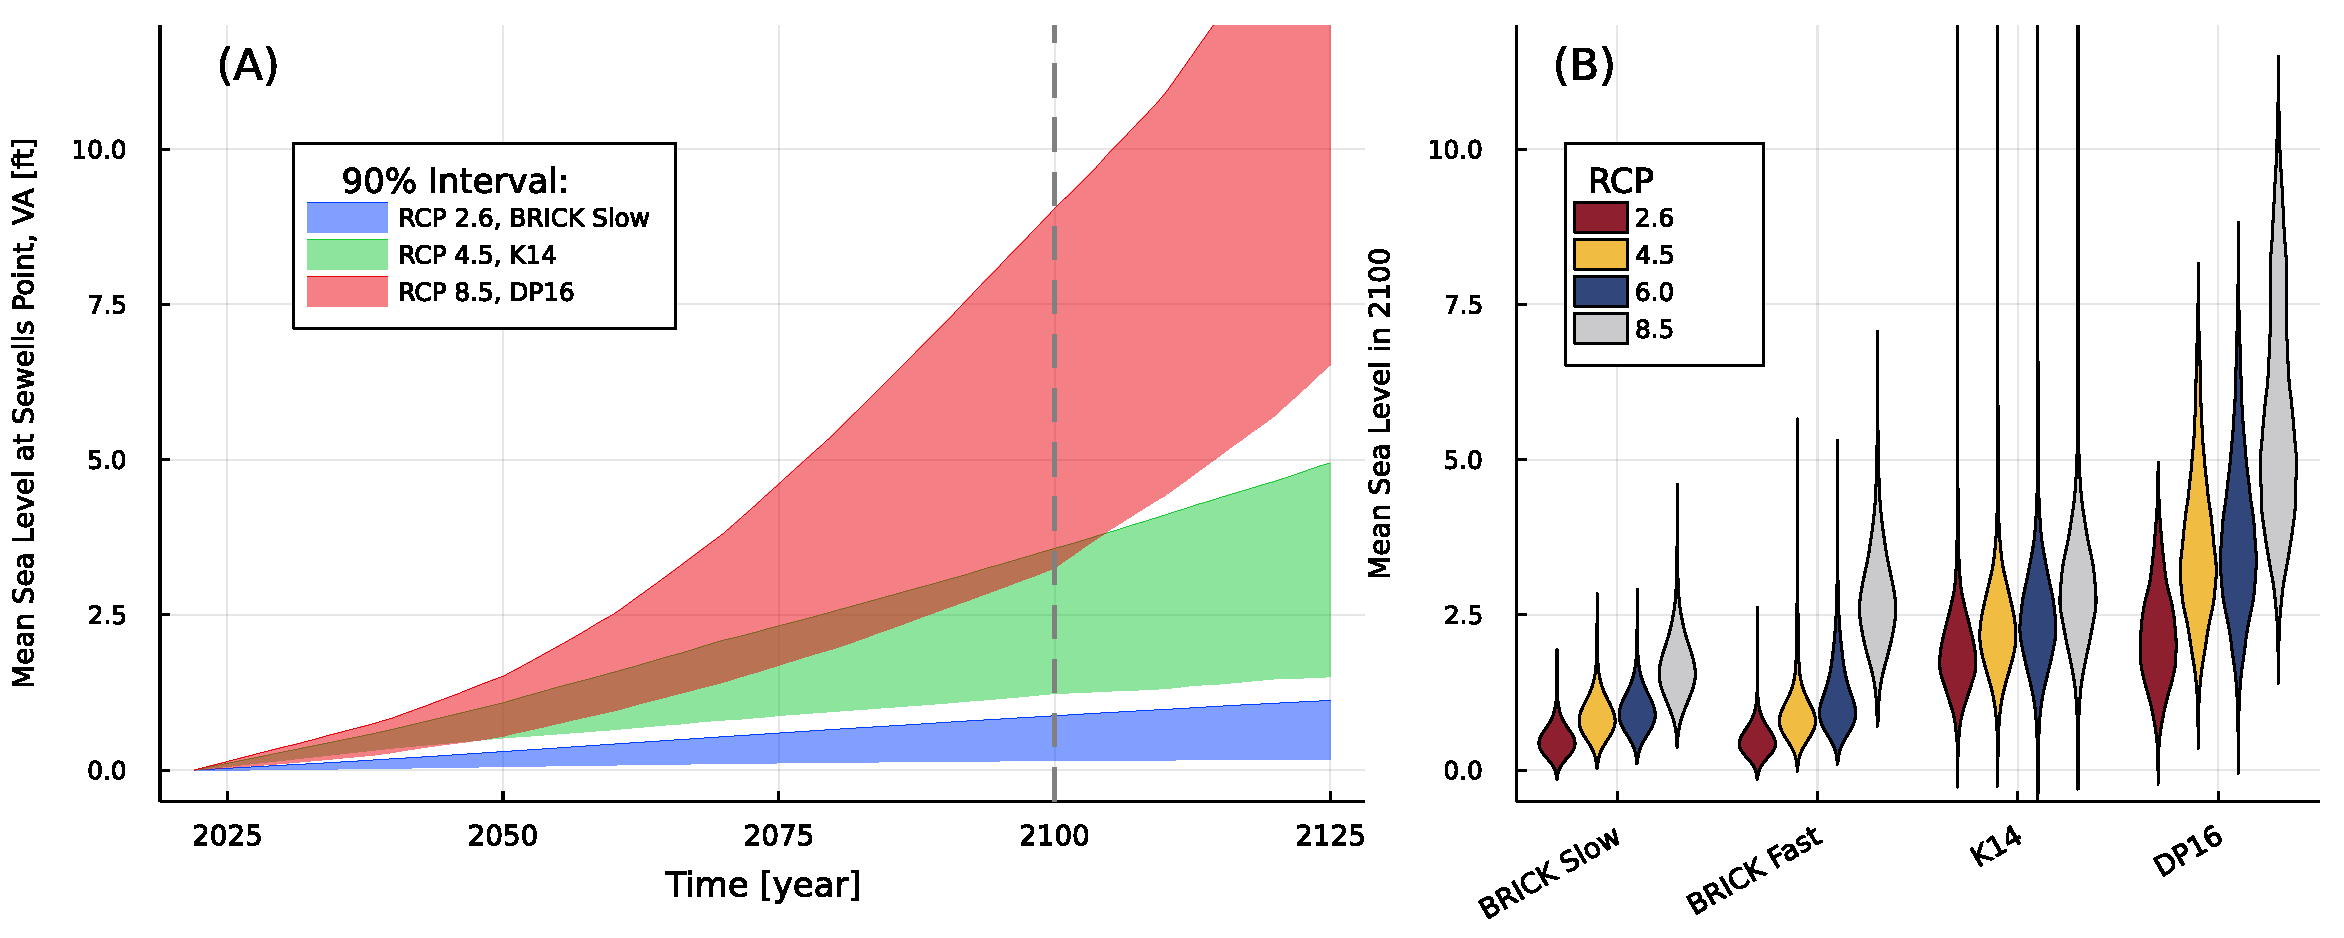
\includegraphics[width=\textwidth]{lsl-evolution}
    \caption{
        Projections of future mean sea level depend strongly on the model (\gls{rcp} scenario and physical representation) used.
        (A): 90\% intervals for mean sea level at Sewells Point, VA as a function of time for a representative subset of three probabilistic models (out of sixteen).
        (B): probability distribution of \gls{msl} at Sewells Point, VA in the year 2100 for each probabilistic model considered.
    }\label{fig:lsl-evolution}
\end{figure}

\Cref{fig:lsl-evolution}(a) shows the time-varying \glspl{pdf} of \gls{msl} for three representative models.
The divergence between the the best-case (blue) and worst-case (red) models is small in the early 21st century and increases rapidly thereafter.
\Cref{fig:lsl-evolution}(b) shows the \glspl{pdf} of mean sea level in 2100 (dashed vertical line in panel (a)) under each of the sixteen models considered.
Both physical model and \gls{rcp} scenario strongly inform the modeled probability distribution.\klaus{Do you want to add a sentence here comparing BRICK to the Kopp et al models?}

\subsection{Storm surges}\label{sec:storm-surge}

Coastal flood hazard does not depend only on \gls{msl} but also on storm surges.
Neglecting hydrodynamics, we model annual maximum floods $y(t)$ as the sum of sea level $\overline{y}(t)$ and annual maximum storm surges $y'(t)$.
In this subsection we describe our representation of storm surge.

Data on storm surge comes from Sewells Point, VA (NOAA gauge 8638610).
The NOAA tides and currents dataset is available to the public at \url{https://tidesandcurrents.noaa.gov/waterlevels.html}.
Hourly recordings of water level are available from 1928 to the present; we use data from the period January 01 1928 to December 31 2021.
For each year we first remove the annual mean, then extract the  maximum water level.
We refer these maxima as the annual maximum storm surges $y'(t)$.

\Cref{fig:surge-obs-return}(a) shows the time series of historical annual maximum storm surges.
Major historical surges have been driven by two different mechanisms: tropical cyclones and nor'easters.
The largest recorded surge was the Chesapeake-Potomac hurricane of 1933, which caused a surge of over \SI{7}{ft} at this gauge, but other hurricanes and nor'easters have caused surges above \SI{6}{ft}.

\begin{figure}
    \centering
    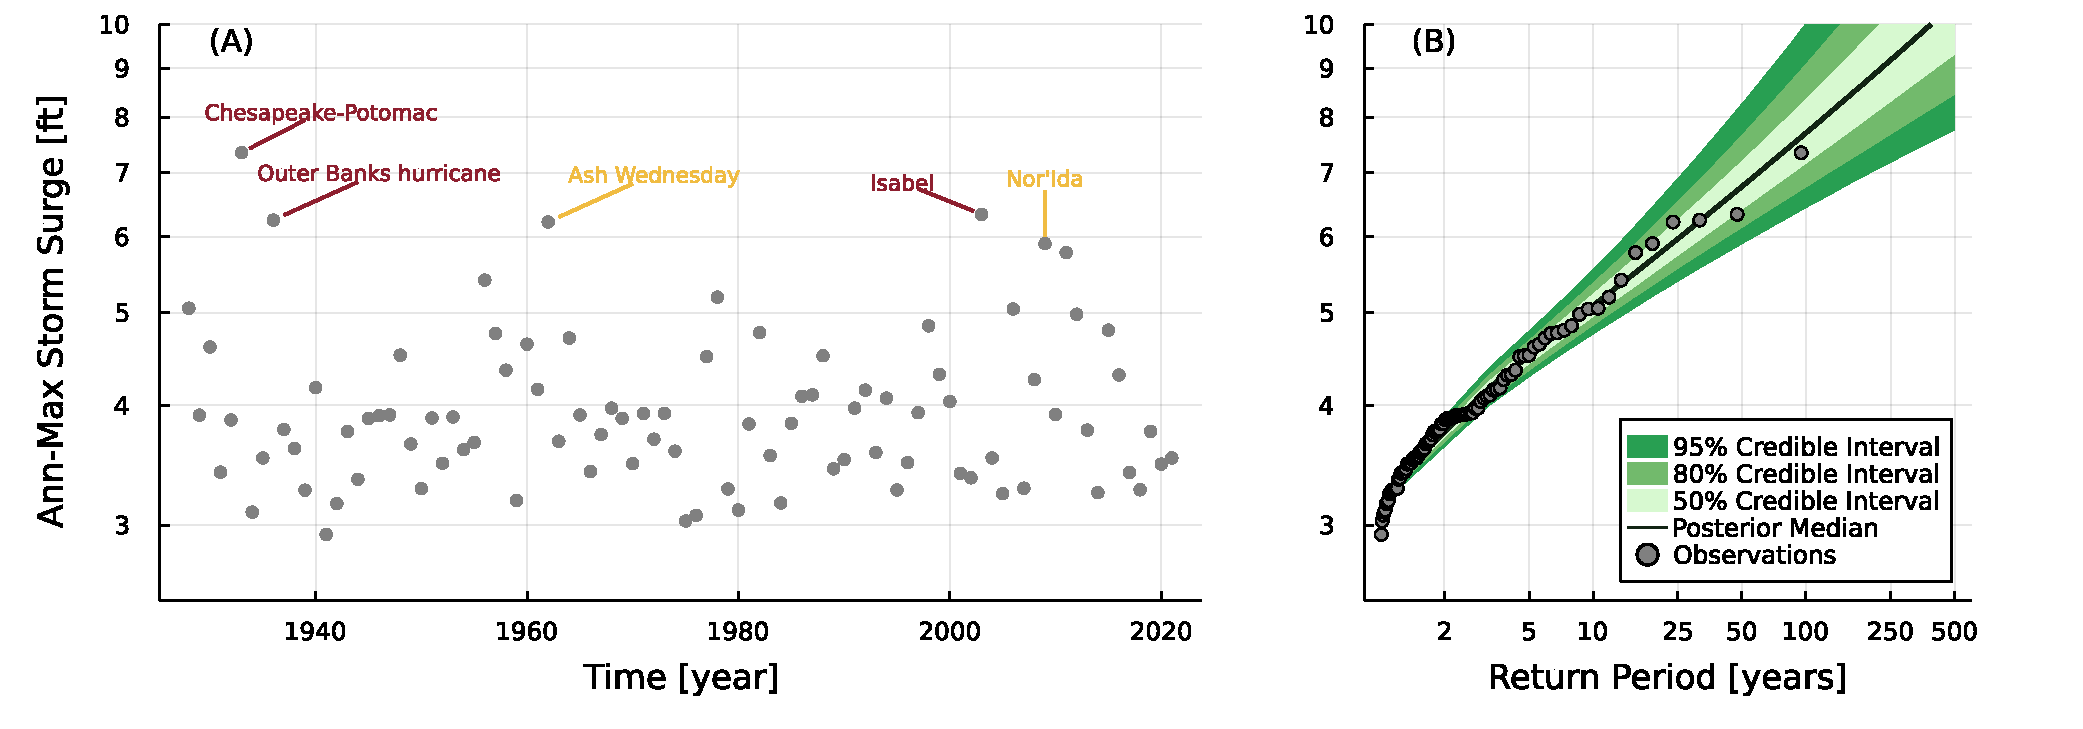
\includegraphics[width=\textwidth]{surge-obs-return}
    \caption{
        Annual maximum storm surges (after subtracting mean sea level) at Sewells Point, VA.
        (A):
        time series of historic storms.
        Red (yellow) arrows denote notable tropical cyclones (nor'easters).
        (B):
        return periods.
        Dots indicate observed values; their $x$-value (``plotting position'') is calculated using the Weibull formula (eq.~\ref{eq:plot-pos}).
        Gray lines show the 50, 80, and 95\% posterior confidence intervals from the Bayesian \gls{gev} fit (\cref{sec:storm-surge}).
    }\label{fig:surge-obs-return}
\end{figure}

We model future storm surge using a stationary \gls{gev} model:
\begin{equation}\label{eq:surge-model}
    y'(t) \sim \text{GEV}\left(\mu, \sigma, \xi \right),
\end{equation}
where $y'(t)$ is the storm surge (above sea level) in year $t$ and $\mu$, $\sigma$, and $\xi$ are the location, scale, and shape parameters, respectively, of the \gls{gev} distribution.
This model is stationary because there is no time dependence; surges in different years are modeled as \gls{iid}.

To improve estimates, we add twp forms of prior information.
First, we constrain $\xi > 0$ to reflect knowledge about the support of $y'$: when $\xi < 0$, $y' \in \qty(-\infty, \mu - \nicefrac{\sigma}{\xi})$  and when $\xi > 0$, $y' \in \qty(\mu-\nicefrac{\sigma}{\xi}, \infty)$.
Since storm surges cannot be negative, only the latter is physically defensible.
Second, we add weakly informative priors.
Rather than applying prior information directly over the joint distribution of the priors $\qty{\mu,\sigma,\xi}$, for which intuition is difficult, we apply a prior over extreme quantiles of the distribution as in \citet{coles_evd:1996}.
Specifically we apply half Normal (\ie, Normal distributions truncated at zero) priors over the 2, 10, 100, and 500 year return levels, with means \SIlist{4;6;10;15}{ft} and standard deviations \SIlist{1.5;1.75;2.25;2.75}{ft}, respectively.
These values were chosen to represent plausible physical ranges and are plotted in \cref{fig:surge-gev-priors}.

For inference, we draw \num{10000} samples from the posterior distribution $p(\mu,\sigma,\xi | y')$ using Hamiltonian Markov Chain Monte Carlo \citep{Betancourt:2017vd,hoffman_nuts:2011} through the Turing package of the Julia programming language \citep{perkel_julia:2019,ge_turing:2018,tarek_dynamicppl:2020,besancon_distributions.jl:2021,bezanson_julia:2012}.
Diagnostics suggest (though cannot guarantee) convergence (see \cref{tab:surge-posterior-mcmc-diagnostics}).
We evaluate the model's fit using posterior predictive checks \citep[see section 2.4 of][and references therein]{gelman_workflow:2020}.
Using the lag 1 and 2 partial autocorrelations, sample maximum, sample minimum, sample median, and Mann-Kendall test value as Bayesisan test statistics, we found that draws from the posterior predictive distribution matched the observed test statistic credibly \cref{fig:surge-test-statistics}.
Since \cref{fig:surge-test-statistics}(b) suggests the possibility of meaningful temporal structure not captured by our stationary \gls{iid} model, future efforts  could represent this structure by conditioning the parameters of the distribution on relevant climate indices \citep[as in][]{wong_structural:2020}.

\Cref{fig:surge-obs-return}(b) shows the estimated return periods for these storm surges.
The return period of the data (dots) is shown using the Weibull (``empirical'') plotting position
\begin{equation}\label{eq:plot-pos}
    \frac{r}{N + 1}
\end{equation}
where $N$ is the sample size and $r$ is the order of the $N$ observations ($r=1$ is the largest, $r=N$ is the smallest).
The good fit of the Bayesian fit (gray shading) to the data (points) suggests that the stationary approximation is reasonable for this dataset.

\subsection{Expected annual damage}\label{sec:ead}

There are two components of the system model (``relationships'' in \cref{fig:xlrm}).
The first is a fragility model that estimates the expected flood loss for a particular year, given the elevation of the house and the mean sea level for that year.
Specifically, we define expected annual damages in year $t$ as the expectation of the damage function with respect to storm surge.
This expectation depends on the house's height ($h = h_0 + \Delta h$) where $h_0$ is the initial height relative to the gauge and $\Delta h$ is the amount by which the house is elevated.
The expcted annual damage is thus
\begin{equation}\label{eq:ead}
    \textrm{EAD} = \mathbb{E}[D(h-\overline{y})] = \int_{y'} p(y') D(h - (\overline{y} + y')) \dd{y'}
\end{equation}
where $D(h-y)$ is a deterministic function specifying damage as a function of flood depth (relative to the house).
The term $\overline{y}$ in \cref{eq:ead} is time-dependent but we have omitted the time dependence for readability.
Following \citet{zarekarizi_suboptimal:2020} we use the we use the Hazard U.S. (HAZUS) depth-damage curves provided by FEMA to parameterize $D(h-\overline{y})$; this depth-damage relationship is shown in \cref{fig:cost-depth-damage}.
For comparison, \cref{fig:cost-depth-damage} also shows results using the ``Europa'' depth-damage relationship developed by the Joint Research Center of the European Commission's science and knowledge service \citep{huizinga_depthdamage:2016}.
Although \citet{zarekarizi_suboptimal:2020} demonstrate that the choice of fragility function is important for informing house elevation, we use only the HAZUS model for concision.

The expected annual damage is sometimes calculated by assuming analytically tractable functional forms for the depth-damage relationship and for the  distribution of hazard \citep[\eg][]{vandantzig_dike:1956}.
However, the convolution of the HAZUS depth-damage equation with the \gls{gev} posterior does not have a tractable analytic solution so we instead estimate it through a Monte Carlo method:
\begin{enumerate}
    \item For $k=1, \ldots, K$:
          \begin{enumerate}
              \item sample a draw from the posterior distribution of flood hazard to get $\left\{ \mu_k, \sigma_k, \xi_k \right\}$
              \item simulate a single storm surge from the stationary distribution (\cref{eq:surge-model}) and add the mean sea level to get total flood depth $y^\mathrm{sim}_k$
              \item calculate the flood damages for this draw by plugging the annual maximum flood depth ($h - y_k$) into  the deterministic HAZUS depth-damage relationship, storing this as the $k$th damage.
          \end{enumerate}
    \item Estimate expected annual damages as the sample mean of the $K$ estimates
\end{enumerate}
Evaluating expected annual damages for each of $N$ simulations of sea level rise, each of $J$ draw from the posterior distribution of storm surge, and each of $T$ time steps requires $N \times J \times T \times K$ simulations.
Since $K$ must be large in order to accurately approximate the integral, this requires incurring a heavy computational cost.
However, noticing that this function depends only on the elevation of the house relative to \gls{msl}, we develop a simple emulator for expected annual damages given this difference: $\hat{D}(h - \overline{y})$.
To do this, we  precompute expected annual damage for all height differences in \SI{0.25}{ft} increments from \SIrange{-30}{30}{ft} and fit a piecewise linear interpolation to this data.
We use $K=\num{1e6}$ samples to fit this emulator for each of the 241 increments.
This model is shown in \cref{fig:cost-expected-damage-emulator}.
Once this interpolation has been precomputed, calculating expected annual damage for a particular year only requires evaluating a piecewise linear function.

\subsection{Lifetime expected damages}\label{sec:led}

The second component of the system model converts a time series of annual expected damages (\cref{sec:ead}) into lifetime expected damages, which we define as the up-front cost plus the discounted sum of expected annual damages
\begin{equation}\label{eq:led}
    \textrm{LED} = \sum_{t=1}^T \gamma^{t-1} \mathbb{E}[d_t | \Delta h],
\end{equation}
where the discount rate is $1 - \gamma$.
For the didactic purposes of this study we neglect uncertainty in the discount rate \citep{zarekarizi_suboptimal:2020,arrow_discount:2013} and use a fixed discount rate (see \cref{tab:uncertainties}).
Neglecting uncertainty in house lifetime, we model flood damages over a fixed house lifetime (\cref{tab:uncertainties}).
We calculate lifetime expected damages \emph{for each \gls{sow} separately}.

To assess the performance of a given decision for a specific \gls{sow}, we calculate the following metrics \emph{for each decision-\gls{sow} combination}.
\begin{description}
    \item[up-front cost] is the cost of elevating a house. Following \citet{zarekarizi_suboptimal:2020}, we use estimates of construction cost from the Coastal Louisiana Risk Assessment \citep{fischbach_clara:2012}. We normalize this cost by house value. This cost curve is shown in \cref{fig:cost-up-front}.
    \item[lifetime expected damages] is discussed in \cref{eq:led}
    \item[expected lifetime costs] is the sum of lifetime expected damages and up-front costs
\end{description}

\subsection{Experiment design}

In \cref{fig:flowchart} we introduce a general notation for simulation-based decision analysis.
We consider $J$ \glspl{sow} representing time series of \gls{msl} and $I$ discrete decisions $x_1, \ldots, x_I$ representing the choice for how high to elevate the house.
For each combination of these, we calculate the vector of metrics described in \cref{sec:led}, which we denote $u_{ij} = f(x_i, s_j)$, using a system model $f$.
This system model caculates the metrics $u$ (which in this case is a vector) using the equations and relationships described in the preceding subsections.
We begin in \cref{sec:multiple-simulation} by using the system model to explore the drivers of desirable and undesirable outcomes (blue box in \cref{fig:flowchart}).
Next in \cref{sec:multiple-simulation} we consider scenario-conditional optimization and introduce ``the multiple \gls{pdf} problem'' (red box in \cref{fig:flowchart}).
Finally in \cref{sec:synthesizing} we introduce a metnod for synthesizing uncertainty across the multiple \glspl{pdf} (orange box in \cref{fig:flowchart}).

\begin{figure}
    \centering
    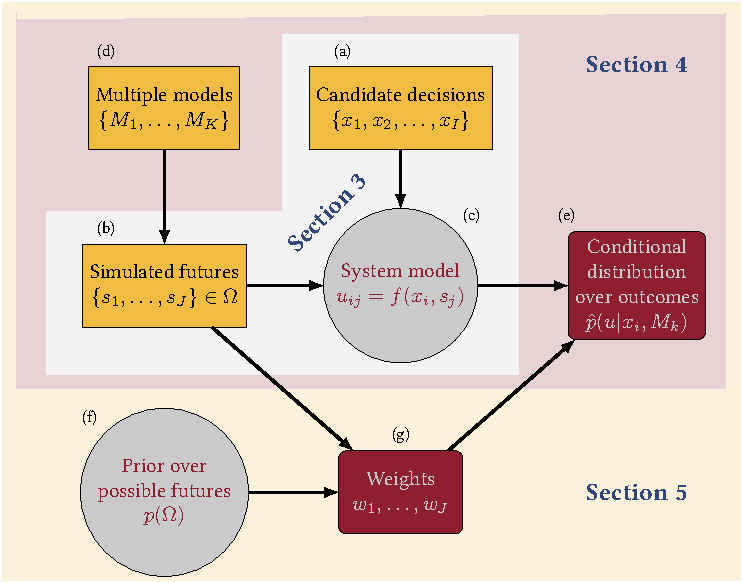
\includegraphics[width=4in]{bayes-rdm.pdf}
    \caption{
        Outline of the proposed decision theoretic framework.
        We begin in \cref{sec:multiple-simulation} using a lens of exploratory modeling (region 1) to analyze the elevation problem.
        Next in \cref{sec:multiple-pdf} we use scenario-conditional probability distributions and the ``multiple \acrshort{pdf} problem'' (region 2).
        Finally in \cref{sec:synthesizing} propose a method for weighting \glspl{sow} to synthesize across multiple \glspl{pdf} (region 3).
    }\label{fig:flowchart}
\end{figure}

\section{Exploratory analysis}\label{sec:multiple-simulation}

We begin by using our model in an ``exploratory'' mode with an aim of learning about interactions between system dynamics and decisions \citep[see][]{bankes:1993}.
Exploratory modeling is used to explore the consequences of different possibilities, and does not require any assessment of how likely a given \gls{sow} may be.

\begin{figure}
    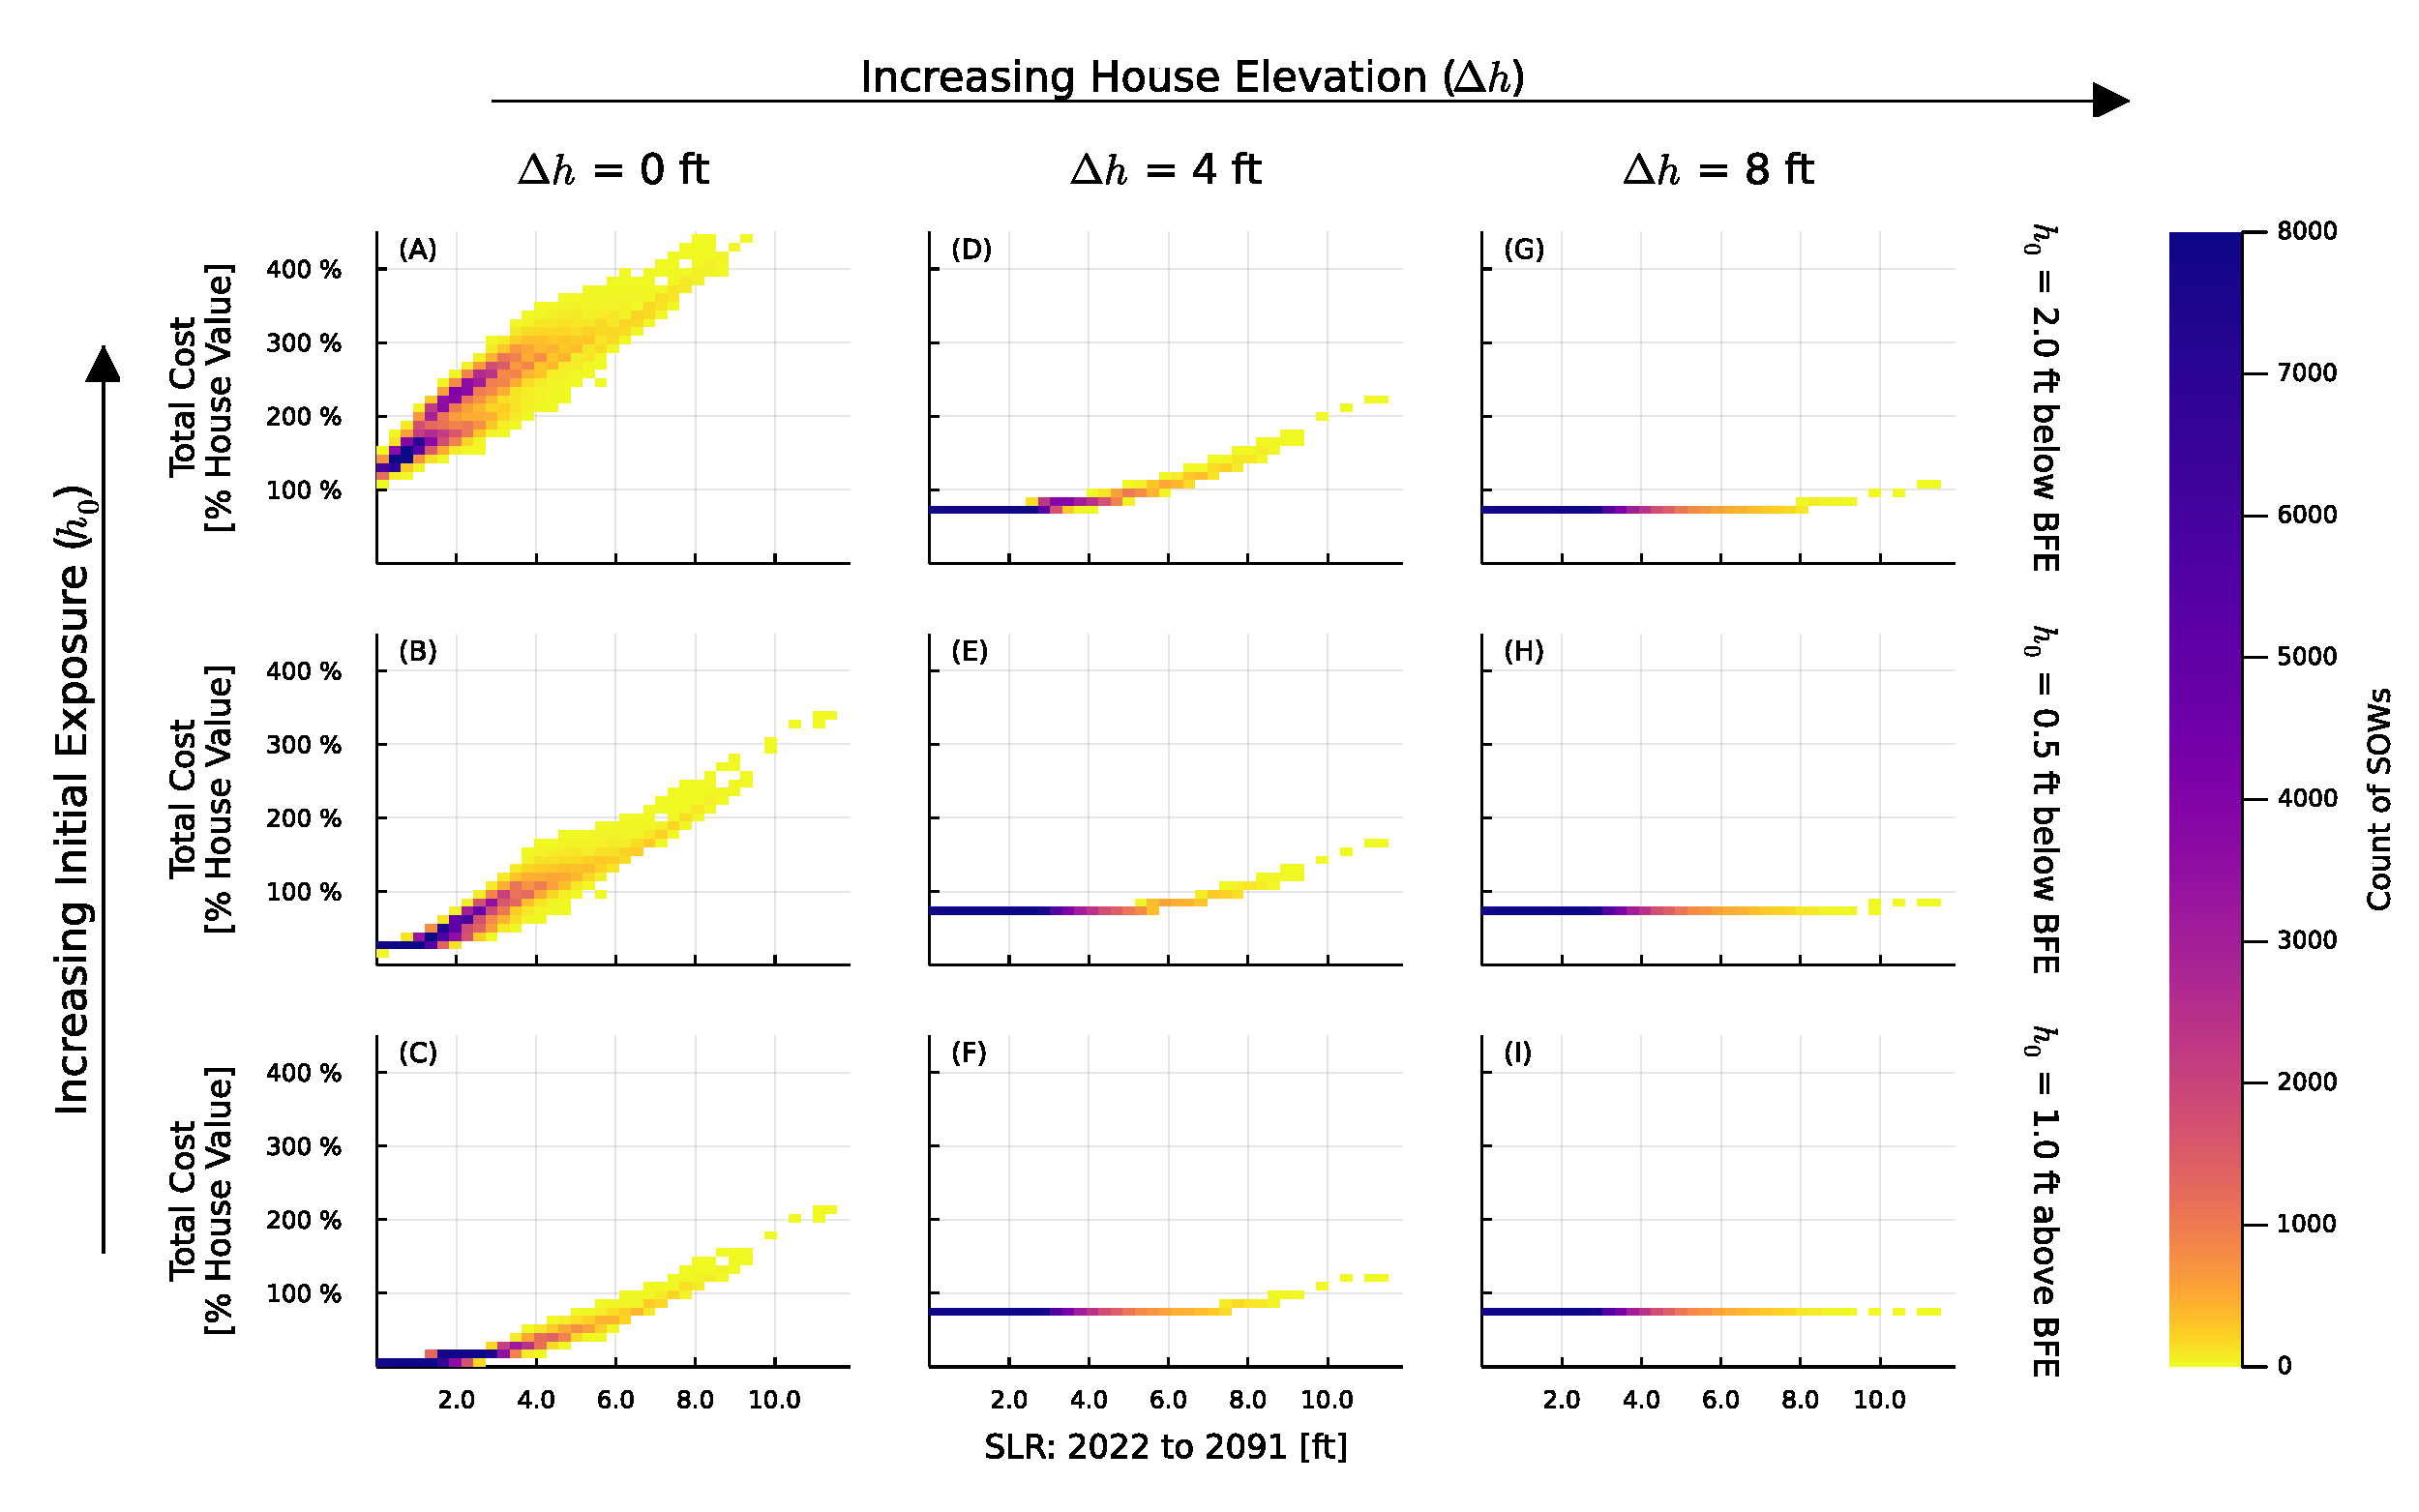
\includegraphics[width=\textwidth]{scenario-map-slr-cost}
    \caption{
        Scenario maps showing the dependence of expected lifetime cost (damages plus up-front cost) as a function of \gls{msl} in 2100 for several values of $\Delta h$ and $h_0$.
        Colors indicate the density of \glspl{sow}; the color of each grid box corresponds to the number of \glspl{sow} falling within that box.
        The lowest-cost outcomes occur when $h_0$ is large, the house is not elevated (no up-front cost), and sea level rise is minimal.
        The highest-cost outcomes arise when the house is not elevated (no up-front cost) and sea level rise is rapid.
        In all cases, elevating the house reduces the variance in total lifetime cost.
        Values are sensitive to model constants; see \cref{tab:uncertainties}.
    }\label{fig:scenario-map-slr-cost}
\end{figure}

\Cref{fig:scenario-map-slr-cost} shows the dependence of expected lifetime costs (damages plus up-front costs) as a function of height increase ($\Delta h$) and sea level rise over the house lifetime.
The best outcomes (yellow) arise when the house is not elevated ($\Delta h = 0$) and sea level rise is minimal (bottom left corners).
The worst outcomes (blue) arise when the house is elevated only slightly and sea level rise is rapid.
As $\Delta h$ increases, the best-case scenario becomes more expensive because up-front costs increase, but worst-case scenarios become less expensive because even if sea level rise is substantial, damages will be negligible.
Decisions about if and, if so, how high to elevate may thus depend on the decision-maker's risk aversion.
Additionally, since exploratory modeling does not shed light on the likelihood of different \glspl{sow}, decisions about if and, if so, how high to elevate will also depend on an assessment of sea level rise likelihoods.

\section{Scenario-conditional probabilistic analysis: the multiple PDF problem}\label{sec:multiple-pdf}

The exploreatory analysis of the previous subsection considered each realization of future sea level to be an exploratory sample from the space of possible futures.
An alternative interpretation of the available \glspl{sow} is as \gls{iid} draws from each of the sixteen models of sea level rise, as shown in \cref{fig:lsl-evolution}.
This has the approach of a probabilistic interpretation: \emph{conditional on a particular model} (\gls{rcp} scenario and ice sheet model structure), we can view corresponding \glspl{sow} as \gls{iid} draws from the distribution of outcomes.

A more formal notation is introduced in boxes (d) and (e) of \cref{fig:flowchart}.
Specifically, for each of $K=16$ models, the samples of metrics are taken to be \gls{iid} samples from the distribution of outcomes (box e).
Since we define these models to estimate $p(\Omega)$, our models $M_1, \ldots, M_K$ return a probability of $1 / J_K$ for each of the $J_K$ simulations from the $K$th model, and $0$ for simulations from all other models.
We can then use this conditional distribution over outcomes to create metrics that depend only on the decision, such as averages or quantiles of outcomes.

\begin{figure}
    \centering
    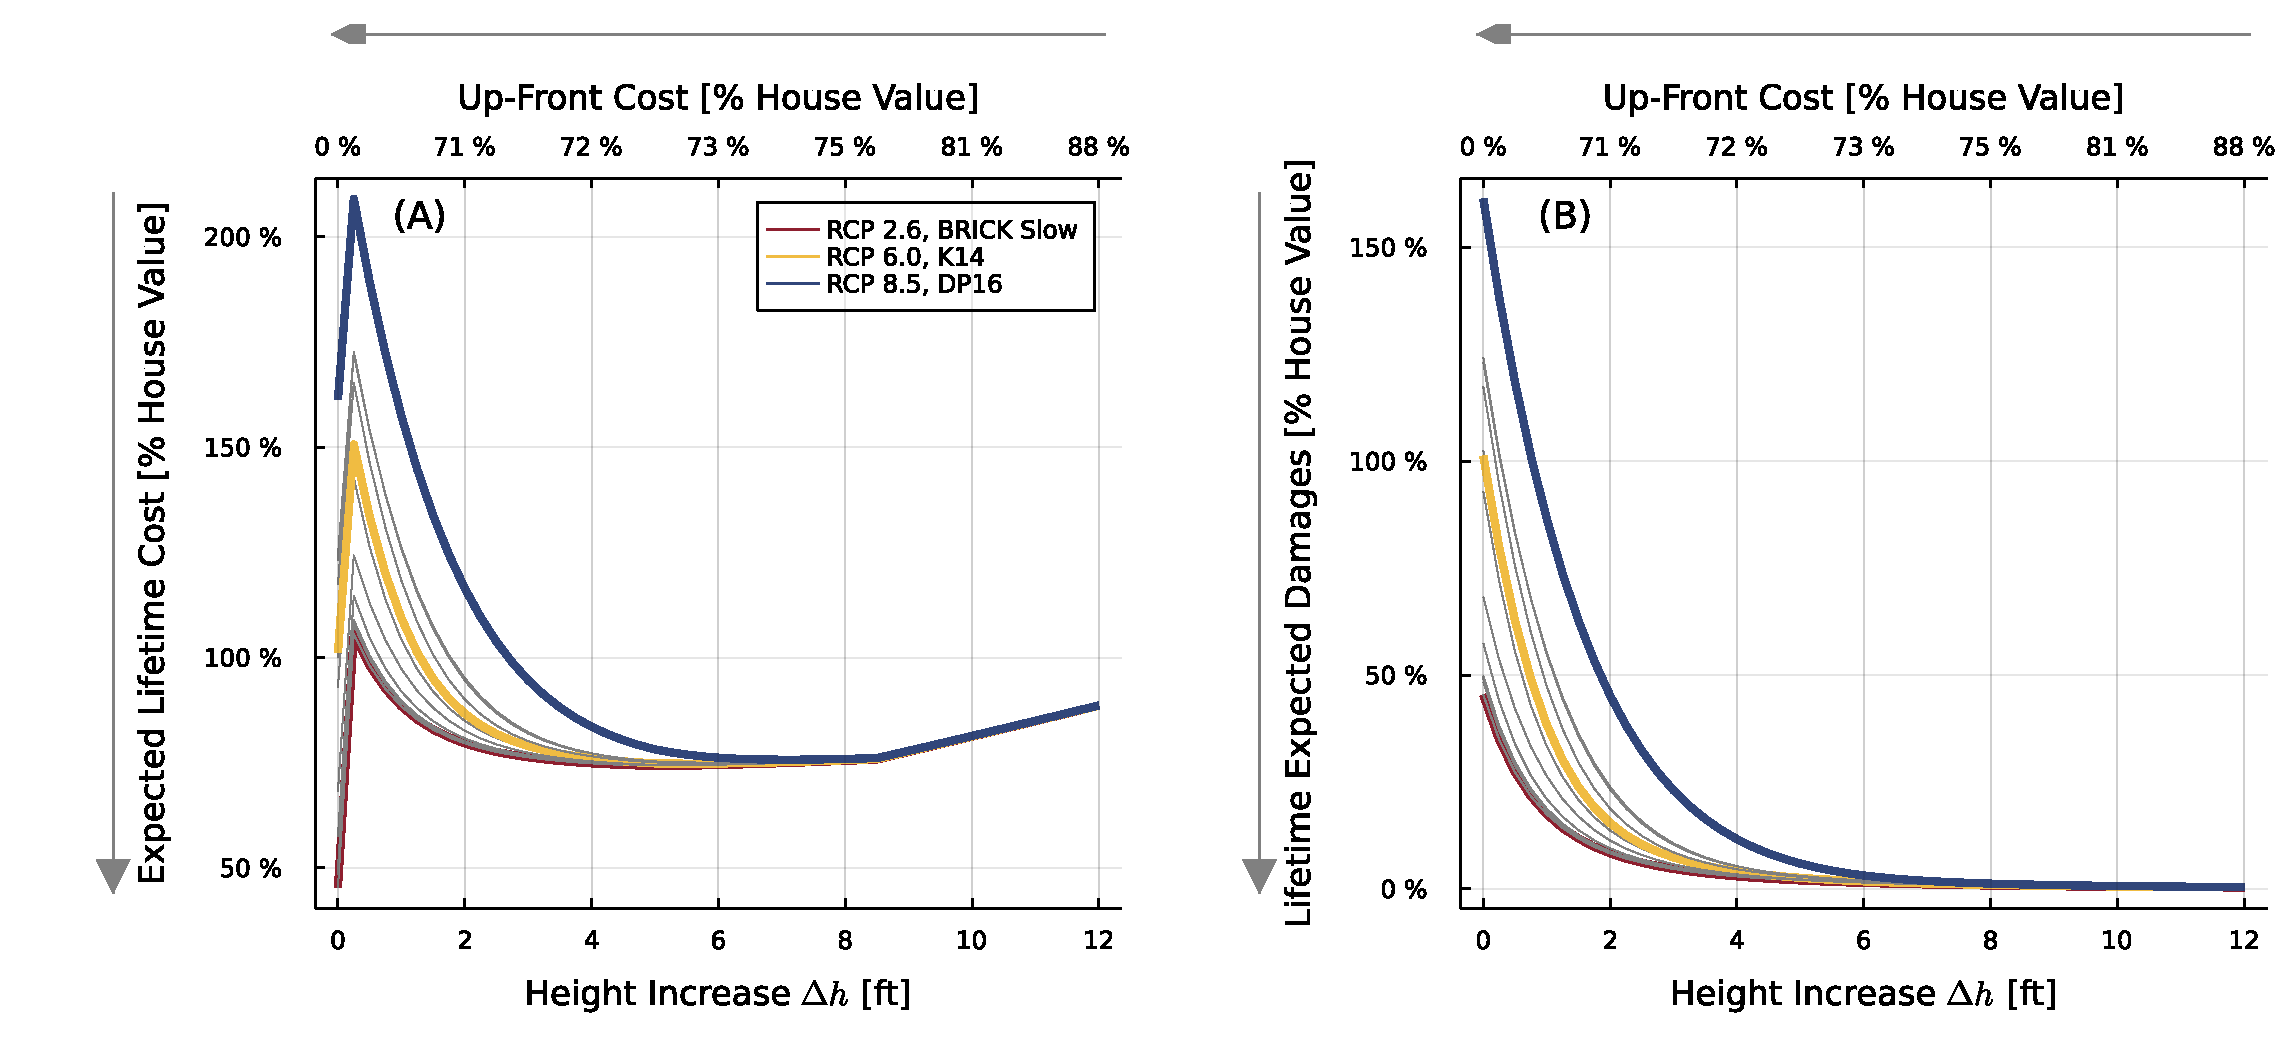
\includegraphics[width=\textwidth]{tradeoffs-by-rcp}
    \caption{
        Each probabilistic model or scenario leads to a different estimate of the Pareto frontier.
        (A): trade-off between up-front cost (which is a monotonic function of height increase) and expected lifetime costs.
        (B): trade-off between up-front cost and lifetime expected damages (eq.~\ref{eq:led}).
        Light gray lines show estimates for all 16 models (four \gls{rcp} scenarios times four physical parameterizations) considered.
        Colored lines highlight three representative models for emphasis.
    }\label{fig:tradeoffs-by-rcp}
\end{figure}

For example, \cref{fig:tradeoffs-by-rcp}(a) plots the total lifetime cost as a function of $\Delta h$ the sixteen models considered (three are highlighted).
Similarly, \cref{fig:tradeoffs-by-rcp}(b) plots the lifetime expected damages.
This figure shows that for small $\Delta h$, expected costs are low under optimistic models (\eg, \gls{rcp} 2.6 with slow ice sheet dynamics) and high under pessimistic models (\eg, \gls{rcp}8.5 with the DP16 model).
Consistent with \cref{fig:scenario-map-slr-cost}, the variability of lifetime costs decreases as $\Delta h$ increases.
Once $\Delta h$ reaches \SIrange[]{3}{7}{ft}, depending on the model considered, construction costs start to dominate flood losses, and thus higher values of $\Delta h$ increase average lifetime costs.

Calculating either of the quantities shown in \cref{fig:tradeoffs-by-rcp} requires synthesizing across \glspl{sow}.
However, these metrics are necessarily dependent on the model used (\ie, \gls{rcp} scenario and model of ice sheet dynamics).
This means that any assessment of decision performance (\eg, an optimal strategy, a Pareto frontier, or a cost-benefit analysis) is conditional upon an (explicit or implicit) model of future outcomes.
Where these models are implicit, they should be made more explicit to facilitate iterative model critique and improvement.

Second, this approach presents what we call ``the multiple \gls{pdf} problem'' because it leaves decision makers with many probability distributions from which to choose.
The multiple \gls{pdf} problem has been shown in other contexts.
For example, \citet{sharma_rcp:2021} modeled the reliability of stormwater infrastructure under different climate models and downscaling methods, finding diverging estimates of future rainfall hazard, even under a single \gls{rcp} scenario.
Although this scenario-conditional analysis is appropriate for understanding differences between models, its key limitation is that \emph{it places the burden for deciding which model to design for onto the end user.}
Further, once a model is chosen, it will under-represent total uncertainty, since this depends on both with- and between-model variability.

\section{Synthesizing PDFs for decision relevance}\label{sec:synthesizing}

\citet{schneider_scenarios:2002} wrote, in the context of \gls{ipcc} assessments, that ``if we in the scientific assessment business do not offer some explicit notions of the likelihood of projected events, then the users of our products -- policy analysts and policy makers -- must guess what we think these likelihood estimates are.''
Motivated by the multiple \gls{pdf} problem, we develop in this section a framework for synthesizing information across \glspl{pdf} using subjective Bayesian modeling.

\subsection{Re-weighting}

Specifically, we frame the set of \glspl{sow} through a sampling lens and consider the possibility that the distribution from which they are sampled, $p_\textrm{sampling}(\Omega)$, does not reflect our subjective belief about their true distribution, $p_\mathrm{belief}(\Omega)$.
Indeed, this is often by design: it is often advantageous to sample low-probability but high-consequence \glspl{sow} to learn about a system's behavior \citep{bankes:1993}.
To address this, we apply a scheme to weight each \gls{sow} based on $p_\mathrm{belief}(\Omega)$.
First, we project the \glspl{sow} $s_1, \ldots, s_J$ onto a one-dimensional representation, which we denote $\psi_1, \ldots, \psi_J$.
As discussed in \citet{csillery_abc:2010} and other research on approximate Bayesian computation, the choice of summary statistic is an important one.
We take the summary statistic to be sea level rise from 2022 to 2100, recognizing that future work could consider multidimensional summaries.

Without loss of generality, we assume the $\psi_j$ to be sorted from least to greatest so that $\psi_{j-1} \leq \psi_j$, ($j \neq 1$).
This allows us to define $p_\mathrm{belief}(\psi \in \Psi)$ instead of $p_\mathrm{belief}(s \in \Omega)$.
Defining $F_\mathrm{belief}(s)$ to be the cumulative distribution corresponding to $p_\mathrm{belief}$, \ie
$$
    F_\mathrm{belief}(\psi) = \int_{-\infty}^{s'} p_\mathrm{belief}(\psi) \dd{\psi},
$$
we calculate weights using \cref{eq:weights} as illustrated in \cref{fig:grid-sketch}.
\begin{equation}\label{eq:weights}
    w_j = \begin{cases}
        j = 1     & F_\mathrm{belief}\qty(\frac{1}{2}\qty[\psi_1 + \psi_2])                                                                   \\
        1 < j < J & F_\mathrm{belief}\qty(\frac{1}{2}\qty[\psi_{j} + \psi_{j+1}]) - F_\mathrm{true}\qty(\frac{1}{2}\qty[\psi_{j-1} + \psi_j]) \\
        j = J     & 1 - F_\mathrm{belief}\qty(\frac{1}{2}\qty[\psi_{J-1} + \psi_J]).
    \end{cases}
\end{equation}

TODO\james{This paragraph needs some work}
The key point to get across is what a subjective belief means in the Bayesian context \citep{savage:1954,gelman_philosophy:2013,gelman_subjectiveobjective:2017}.
David Spiegelhalter had a nice comment on a podcast where he explained that in medicine, there isn't a ``true'' probability that, for example, you will get cancer; this is not some real quantity that can be measured \citep[hence the famous ``probability isn't real'' admonisment of][]{definetti_probability:1972}.
Similarly, the probability distribution of sea level rise in 2100 isn't something that can be measured.
However, probability provides a clear and self-consistent mathematical language for reasoning about uncertainty, which is why we're using it.
A key advantage is that \textbf{since we can't be right, we can at least be transparent} about the assumed values of sea level in 2100, rather than hiding behind implicit assumptions.
Thus we refer to the $M_k$ here as \emph{priors} to reflect that they consistently represent our current knowledge.

\begin{figure}
    \centering
    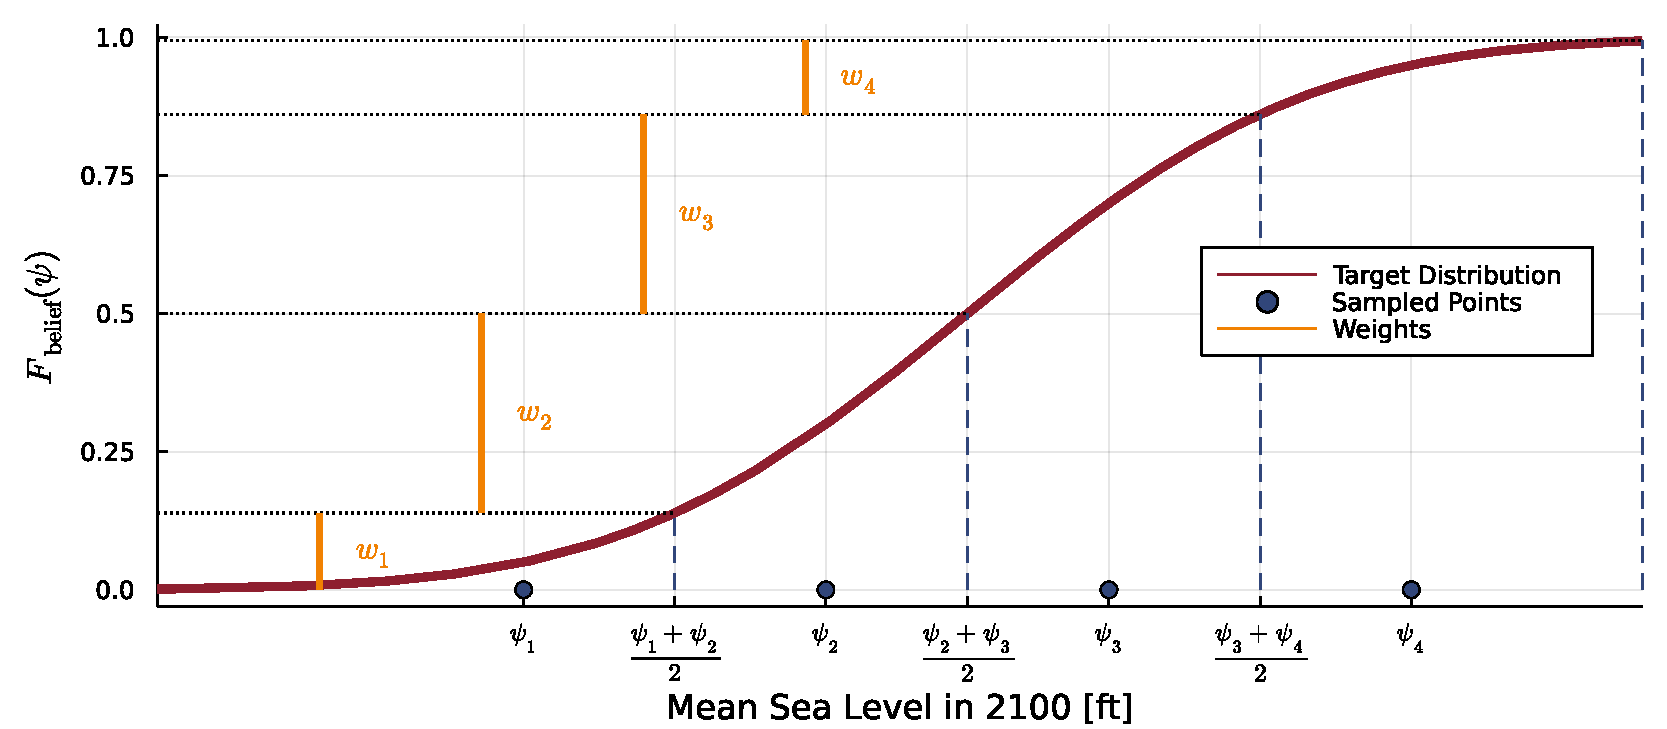
\includegraphics[width=\textwidth]{grid-sketch}
    \caption{
        Schematic of \gls{sow} weighting scheme defined in \cref{eq:weights} for $J=4$.
        This method is illustrated for a hypothetical target distribution (orange line) and four samples $\psi_1, \psi_2, \psi_3, \psi_4$ (blue dots).
        As shown in \cref{eq:weights}, the weights $w_j$ (vertical blue lines) are calculated based on the \gls{cdf} of the target distribution at the halfway points $\frac{1}{2}\qty[\psi_i+\psi_{i+1}]$ (vertical dashed lines).
    }\label{fig:grid-sketch}
\end{figure}

Need to explain how we came up with our two or three subjective priors.\klaus{Are there published assessments we should refer to}
Another advantage of this method is that it is computationally cheap to re-weight the \glspl{sow}.
Thus, exploring performance under alternative priors is computationally cheap and easy to implement.
\Cref{fig:tradeoffs-by-prior} shows the priors used in panel (a) and in panel (b) shows average lifetime cost as a function of the decision ($\Delta h$) after integrating over all possible \glspl{sow} (\ie, after synthesizing the ``multiple \glspl{pdf}.'')

\subsection{Implications}

\begin{figure}
    \centering
    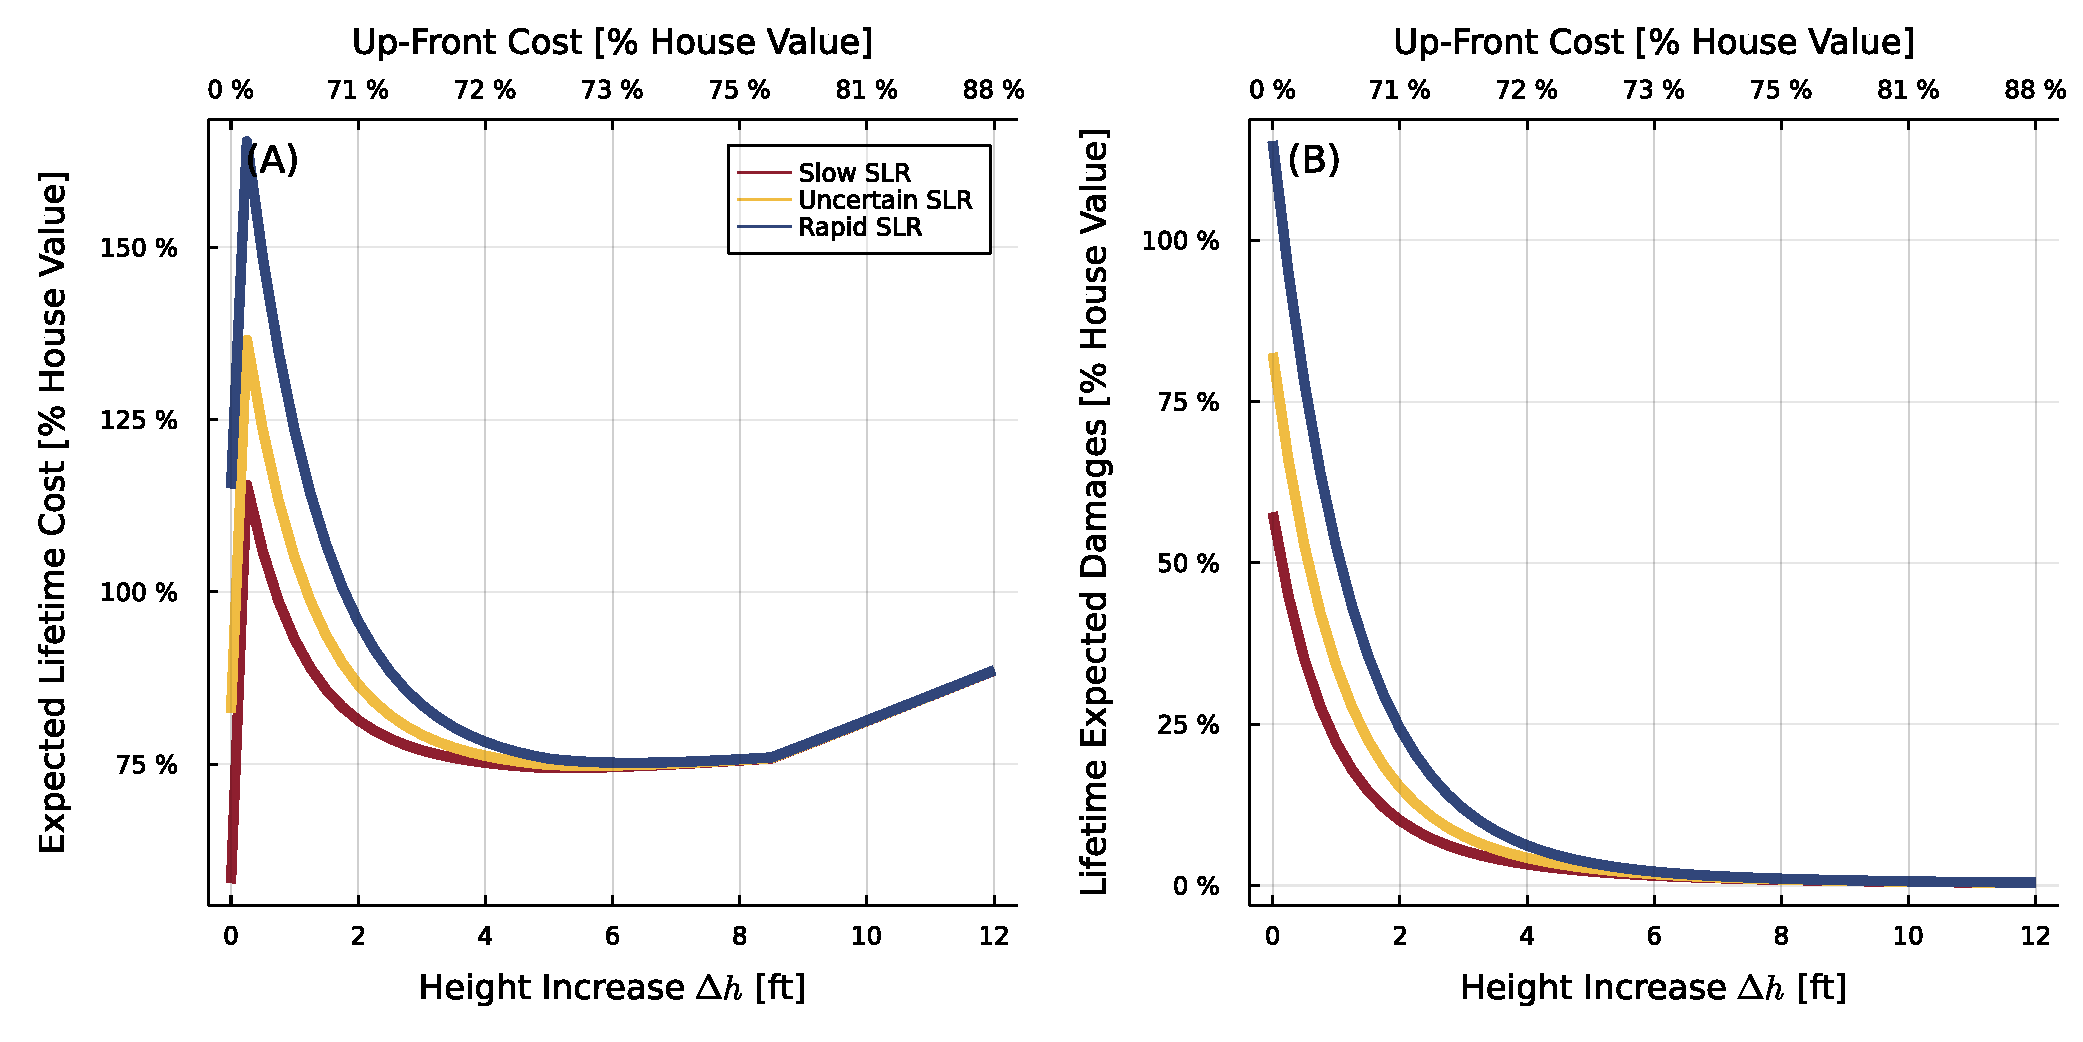
\includegraphics[width=\textwidth]{tradeoffs-by-prior}
    \caption{
        As \cref{fig:tradeoffs-by-rcp}, but Pareto frontiers are shown for the synthesizing Bayesian models.
    }\label{fig:tradeoffs-by-prior}
\end{figure}

This technique can also be used as a diagnostic tool.
In \cref{fig:lsl-priors-weights}, we can see that the ``Pessimistic'' (``Optimistic'') prior heavily weights \gls{rcp} 8.5 (2.6), which is unlikely given current policies \citep{hausfather_scenarios:2020}.\james{Discuss a bit more}


\begin{figure}
    \centering
    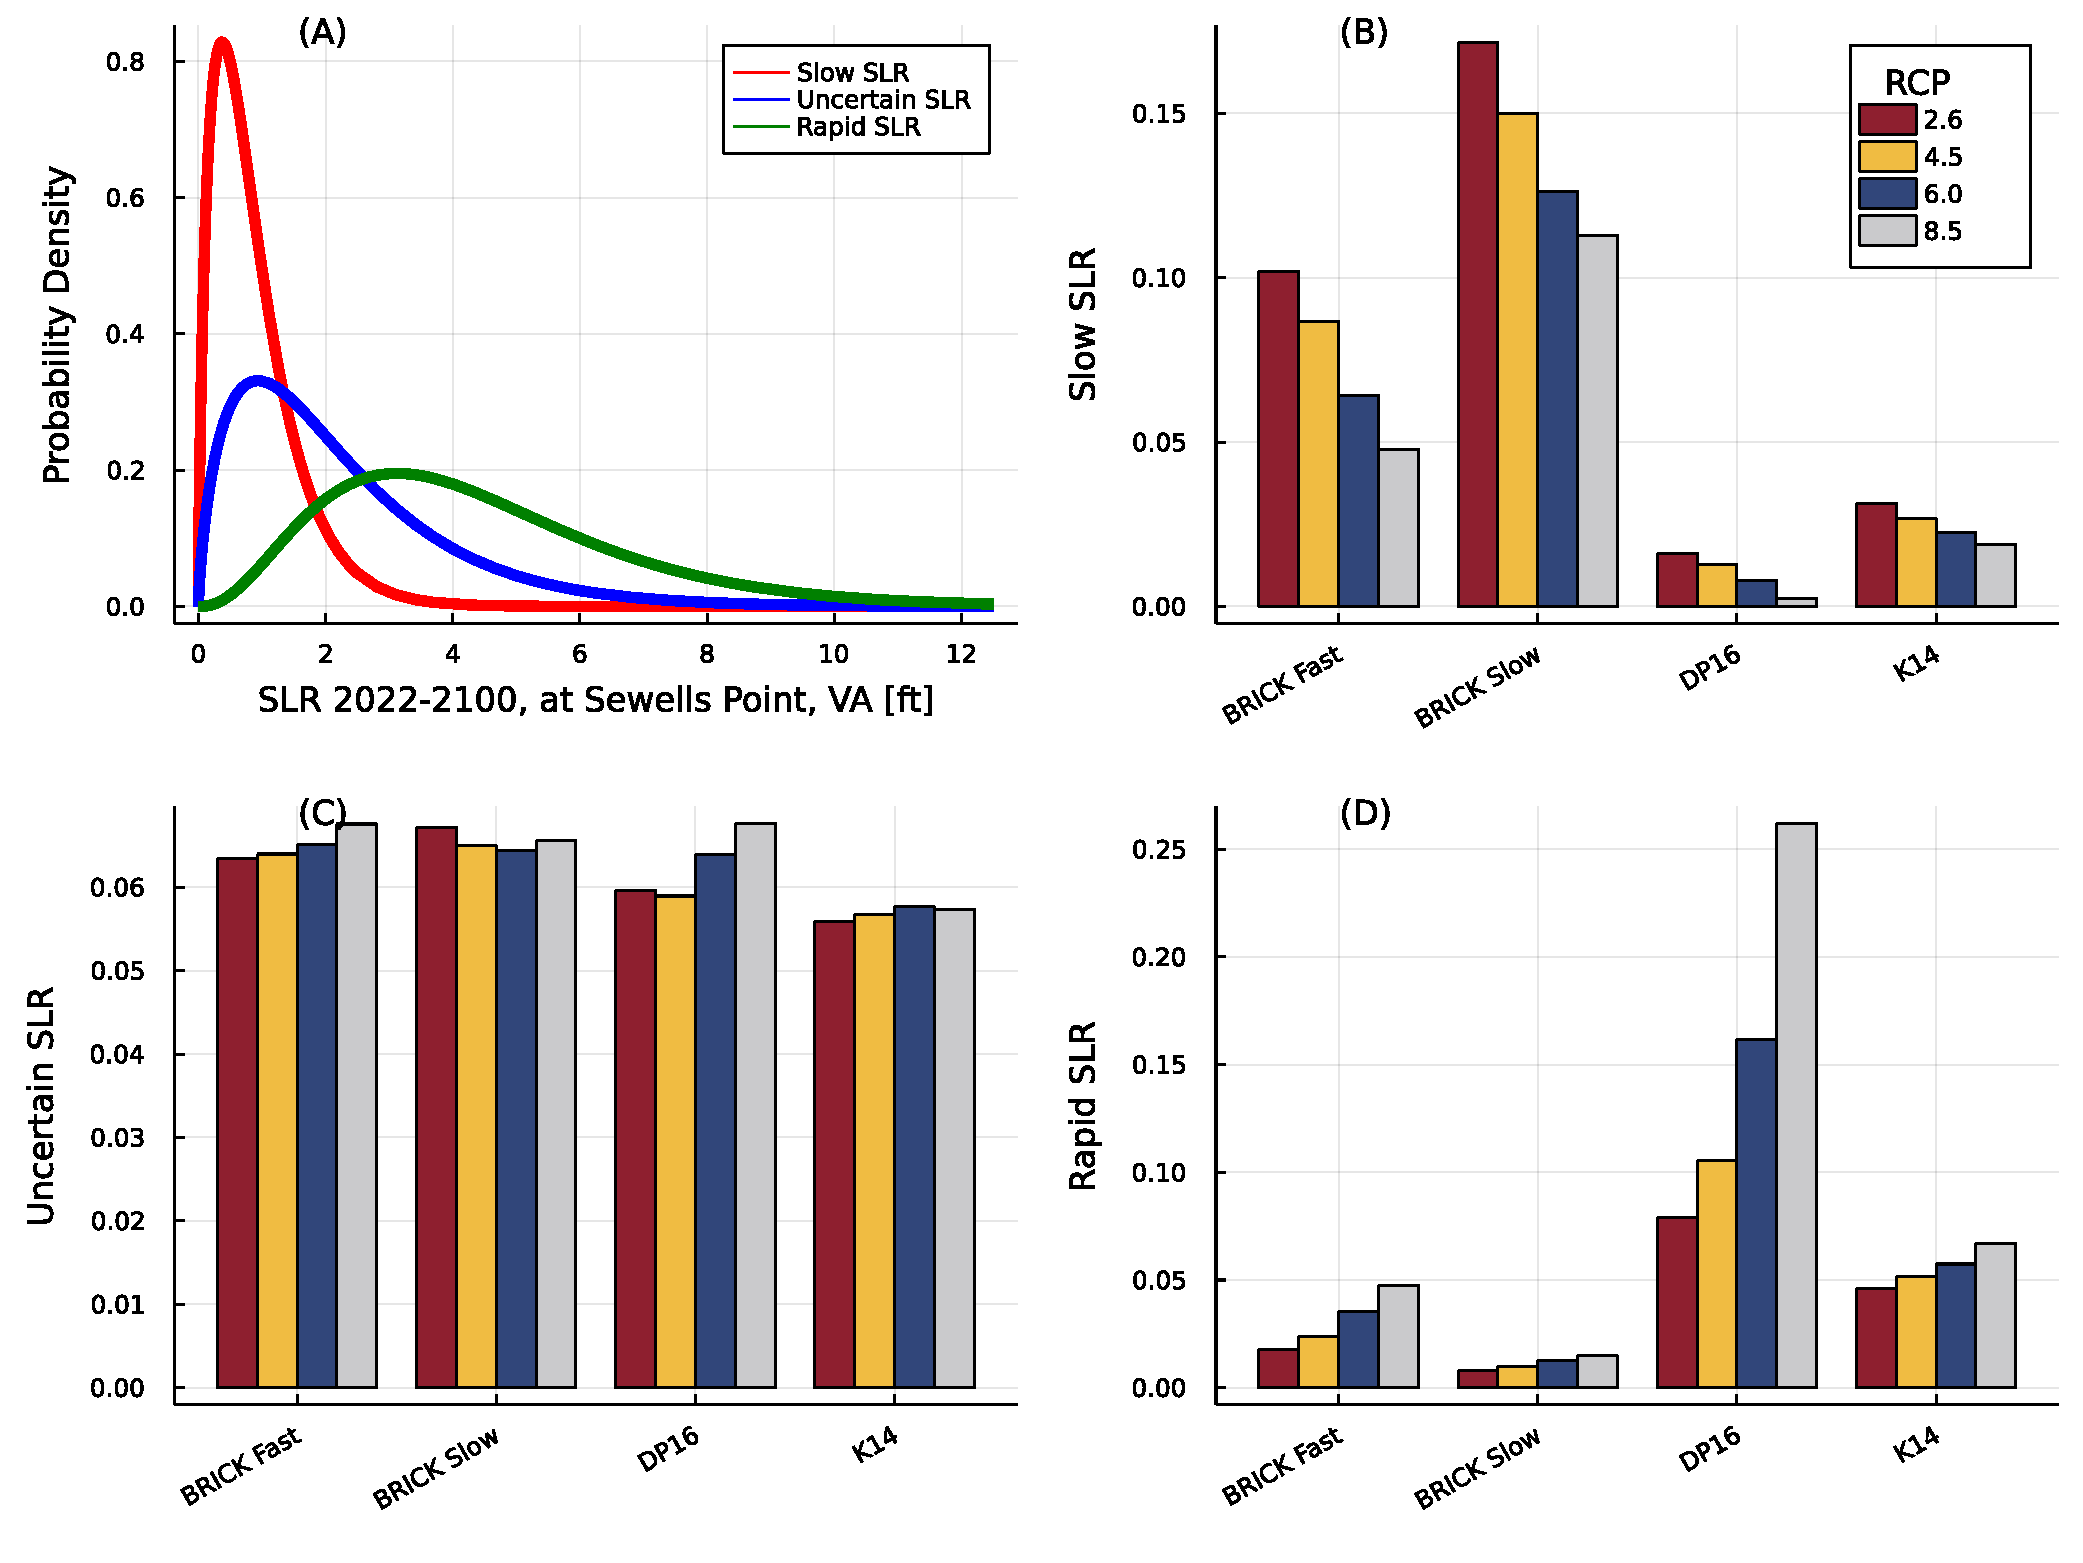
\includegraphics[width=\textwidth]{lsl-priors-weights}
    \caption{
        Subjective priors for local sea level.
        We develop three distributions (``subjective priors'') representing plausible probabilistic beliefs about \gls{lsl} at Sewells Point, VA in 2100, relative to the present.
        The \glspl{pdf} of these subjective priors are shown in panel (A).
        In panels (B-D), we show the relationship between these subjective priors and the 16 probabilistic models (four \gls{rcp} scenarios and four physical representations) available.
        Specifically, (B-D) show the average weight given to each model by each of the three subjective priors.
        The ``Slow SLR'' prior (B) places large weight on BRICK model \citep{wong_brick0.2:2017}, particularly the scenarios with no fast ice sheet dynamics and on low-emissions scenarios.
        The ``Intermediate SLR'' (C) prior places approximately equal weight on all models.
        The ``Fast SLR'' prior (D) places most of its weight on the \citet{deconto_antarctica:2016} model, and in particular on high-emissions scenarios.
    }\label{fig:lsl-priors-weights}
\end{figure}


\section{Discussion and conclusions}\label{sec:conclusions}

Quick summary of what we have done
\begin{enumerate}
    \item OK
\end{enumerate}
Quick summary of what our motivation was
\begin{enumerate}
    \item Explore every \gls{sow}
    \item Be transparent about how we are calculating trade-offs
\end{enumerate}
Philosophical links to Bayesian philosophy and model building in the $\mathcal{M}$-open case (NB: this is copied and pasted from my thesis -- need to rework)
\begin{enumerate}
    \item  \gls{bdt} was conceived as a calculus for reasoning rather than for identifying objective truth; \citeauthor{definetti_probability:1972} often said that ``probability does not exist'' \citeyear{definetti_probability:1972}.
          \citet{savage:1954} and \citet{ramsey_probability:2016}, among others, also viewed probability as ``subjective,'' representing the state of belief of the decision-maker.
    \item The famous phrase ``all models are wrong, but some are useful'' \citep[generally attributed to][]{box:1976} also suggests that probability distributions and predictions ought to be viewed subjectively.
    \item More recent discussions of Bayesian philosophy \citep{jaynes_probability:2003,McElreath:2016vu,Gelman:2014tc,bernardo_bayesian:1994} also emphasize a philosophical view of probability as a language with which to reason about the unknown rather than a statement of objective truth \citep[see][for a thorough discussion of Bayesian philosophy]{gelman_philosophy:2013}.\klaus{Am I reading right that you say ``maybve have this in intro to motivate the analysis?''}
    \item Although the true data generating process is not known and inference should not be represented as objective truth, probability gives a transparent and consistent language for reasoning about uncertainty.\james{This should go to intro}
    \item Since modeling assumptions cannot overcome epistemic uncertainty, even with better models and more data, we draw from the literature on statistical model selection in the $\mathcal{M}$-open setting, which provides a theoretical background for choosing between models when the true data generating process is not among the models considered \citep[see][]{Piironen:2017eh}.\james{Explain this to the audience}
    \item Often, combining inferences from multiple models is more effective than seeking a single ``best'' model \citep{Yao:2018bu}.
          More fundamentally, this literature emphasizes the importance of iteratively building models, simulating the consequences of those models, and critiquing them \citep{gelman_workflow:2020}.
    \item Since, by definition, models are not ``true,'' this iterative workflow aims to identify models that are useful and promote a dialog amongst stakeholders \citep{gelman_philosophy:2013}
    \item Our approach has interesting theoretical links to Bayesian model averaging or stacking \citep{Yao:2018bu}
\end{enumerate}
Links to DMDU literature
\begin{enumerate}
    \item We should also cite \citet{quinn_exploratory:2020}, which makes the point that it matters how you sample \glspl{sow}.
    \item Exploratory modeling can help to demonstrate the existence of particular outcomes, generate hypotheses, build qualitative insight, and identify scenarios worthy of further study \citep[see][]{bankes:1993}.
    \item You can do scenario discovery
    \item We are in effect calculating robustness metrics \citep{mcphail_robustness:2019,herman:2015}
    \item \citet{schneider_scenarios:2002} notes that a RDM analysis ``still requires the construction of ranges of future outcomes -- itself a subjective assessment. Subjectivity is simply inherent in all future projections, whether in natural or social sciences.''
\end{enumerate}

\subsection{Limitations and future work}

Limitations of the case study
\begin{enumerate}
    \item Objectives: real people might care about uncertainty (risk aversion), probability of experiencing flooding at all (disruptions are hard to quantify), usable space created under the house, and more
    \item More uncertainty (damage functions, cost of construction, lifespan, discount rate, \etc)
    \item Better data on cost of elevation and depth-damage
    \item Robustness: ptimize separately for different kinds of house structures and locations
    \item Timing
\end{enumerate}
Limitations of the method
\begin{enumerate}
    \item Our prior $p(\Omega)$ is limited -- we are just using \gls{lsl} in 2100 but we could be looking at more parameters of it including rate of change, \etc
    \item We neglect true ignorance \citep{knight_risk:1921}.\james{Perhaps ``unknown unknowns''}
    \item The real world is in a state of ``unknown unknowns'' \citep[level 5 as defined in][fig.~1]{walker_deep:2013} so trying to represent \emph{all} uncertainty is futile; we must make subjective modeling choices and assumptions about what is most important
\end{enumerate}
Future research needs:
\begin{enumerate}
    \item This didactic example illustrates a need for better synthesis and communication of deep uncertainties for decision making.
    \item More complex models to capture more relevant metrics
    \item Better models of nonstationary hazards
    \item Interacting, sequential decisions
\end{enumerate}

\subsection{Implications}

This approach can be used in many other contexts
\begin{enumerate}
    \item Direct
          \begin{enumerate}
              \item Stormwater management \citep{sharma_rcp:2021,lopez-cantu:2018}
              \item Levee heightening \citep{garner_slrise:2018,oddo_coastal:2017,vandantzig_dike:1956}
          \end{enumerate}
    \item Indirect
          \begin{enumerate}
              \item Lots of economic models like social cost of carbon or effect of policy on metrics of interest make assumptions about deep uncertainties!\james{Let's emphasize this -- really important to policy analysis under deep uncertainty}
              \item Model structure uncertainties
          \end{enumerate}
\end{enumerate}

\section*{End Matter}

\subsection*{Acknowledgements}

This work was supported by the National Oceanic and Atmospheric Administration (NOAA) through the Mid-Atlantic Regional Integrated Sciences and Assessments (MARISA) program under NOAA grant NA16OAR4310179 and by the Penn State Center for Climate Risk Management.
JDG thanks Rice University for support.
KK thanks Dartmouth College for support.
The authors thank Tor Erlend Fjelde for helpful comments.

\subsection*{Code and data availability}

All code, including source code, is available under the GNU Public License (version 3) at \url{https://github.com/jdossgollin/2021-elevation-robustness}.
This code is written in the open source Julia programming language.

\subsection*{Author Contributions}

JDG and KK designed the research.
JDG wrote the codes and ran simulations.
JDG wrote the manuscript with support from KK.
JDG wrote the manuscript in consulation with KK.
JDG and KK revised the manuscript.

\printbibliography

\appendix
\newcommand{\hbAppendixPrefix}{S}
\renewcommand{\thefigure}{\hbAppendixPrefix\arabic{figure}}
\setcounter{figure}{0}
\renewcommand{\thetable}{\hbAppendixPrefix\arabic{table}}
\setcounter{table}{0}
\renewcommand{\theequation}{\hbAppendixPrefix\arabic{equation}}
\setcounter{equation}{0}

\newpage
\section{Supplemental figures}

\begin{figure}
    \centering
    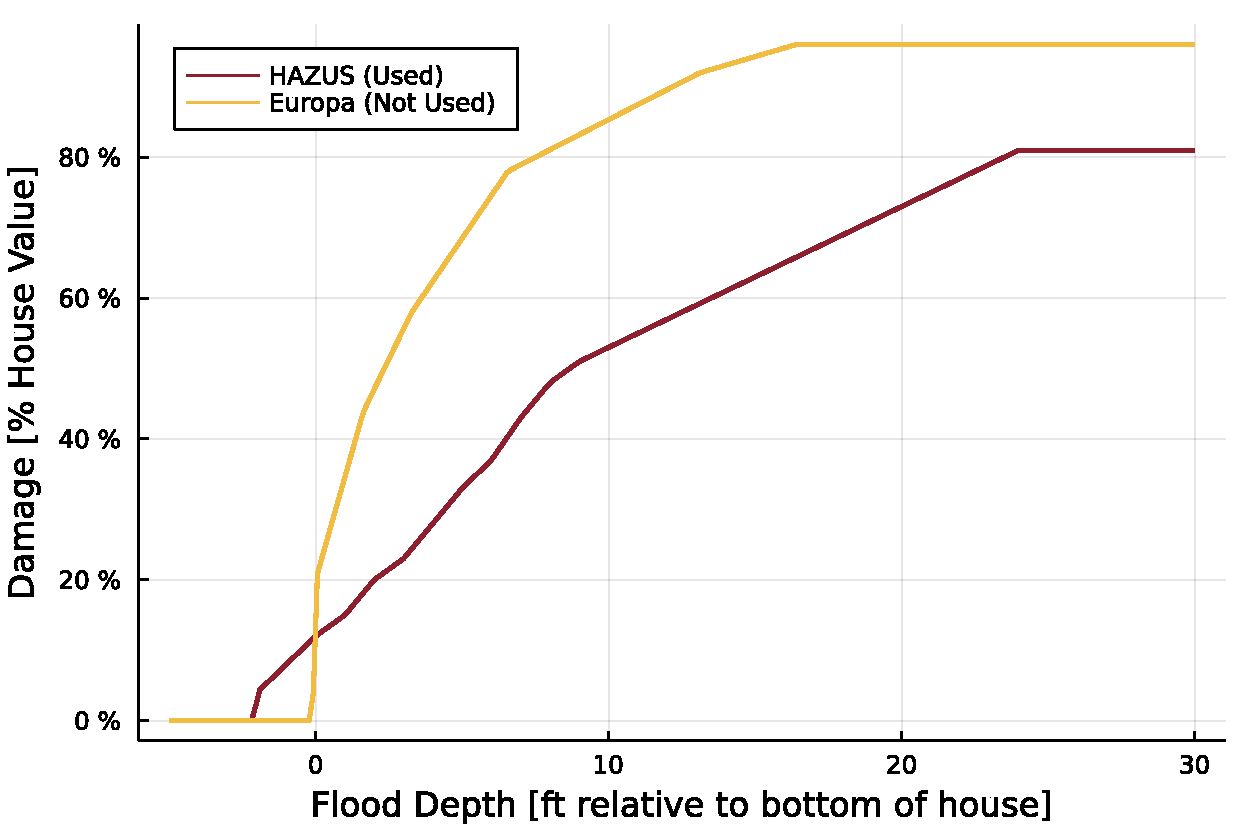
\includegraphics[width=4in]{cost-depth-damage}
    \caption{
        Depth-damage relationship.
        Following \citet{zarekarizi_suboptimal:2020}, we use the Hazard U.S. (HAZUS) depth-damage curves provided by FEMA.
        Since results are sensitive to choice of depth-damage equation, we illustrate (for comparison only) the ``Europa'' depth-damage relationship developed by the Joint Research Center (JRC) of the European Commission's science and knowledge service \citep{huizinga_depthdamage:2016}.
    }\label{fig:cost-depth-damage}
\end{figure}

\begin{figure}
    \centering
    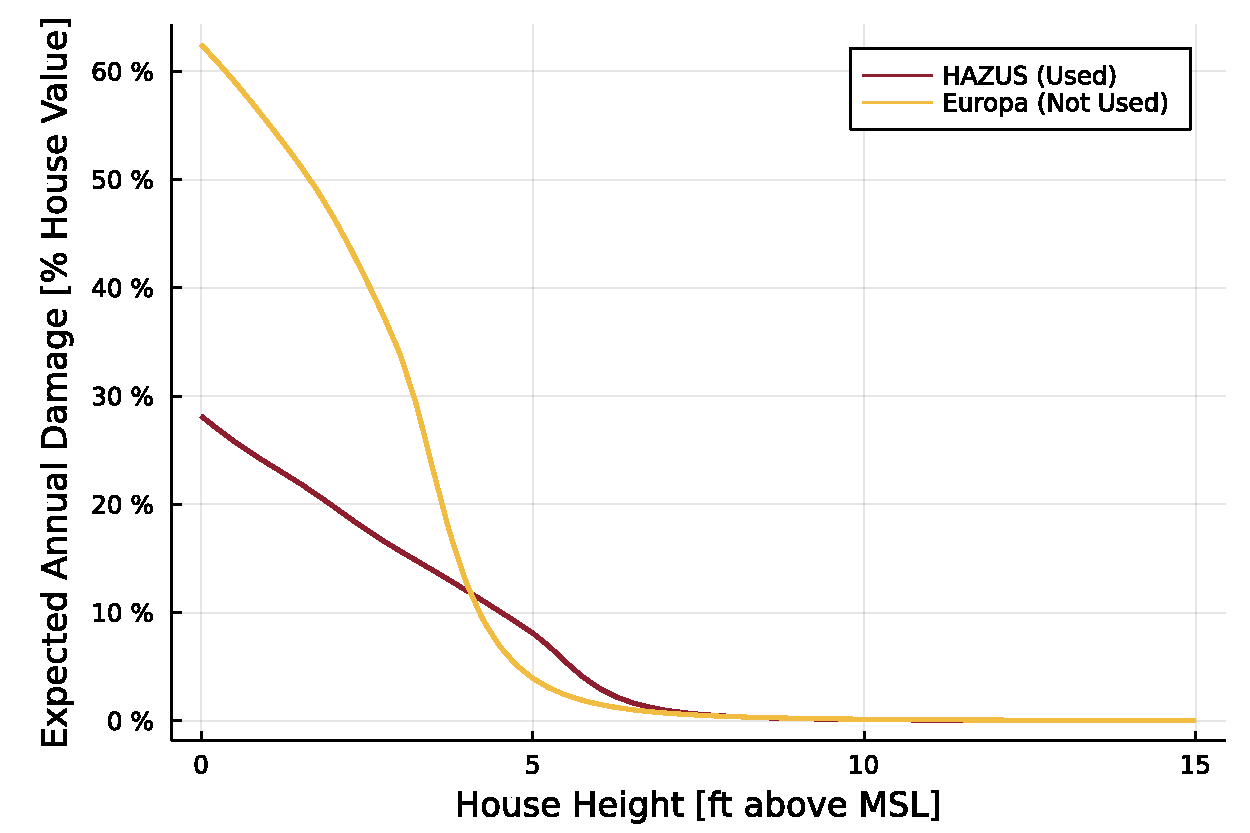
\includegraphics[width=4in]{cost-expected-damage-emulator}
    \caption{
        As discussed in \cref{sec:ead}, we model expected annual damages (eq.~\ref{eq:ead}) as a function of the house's elevation relative to \gls{lsl}.
        Damages ($y$ axis) are shown as a percentage of house value.
    }\label{fig:cost-expected-damage-emulator}
\end{figure}

\begin{figure}
    \centering
    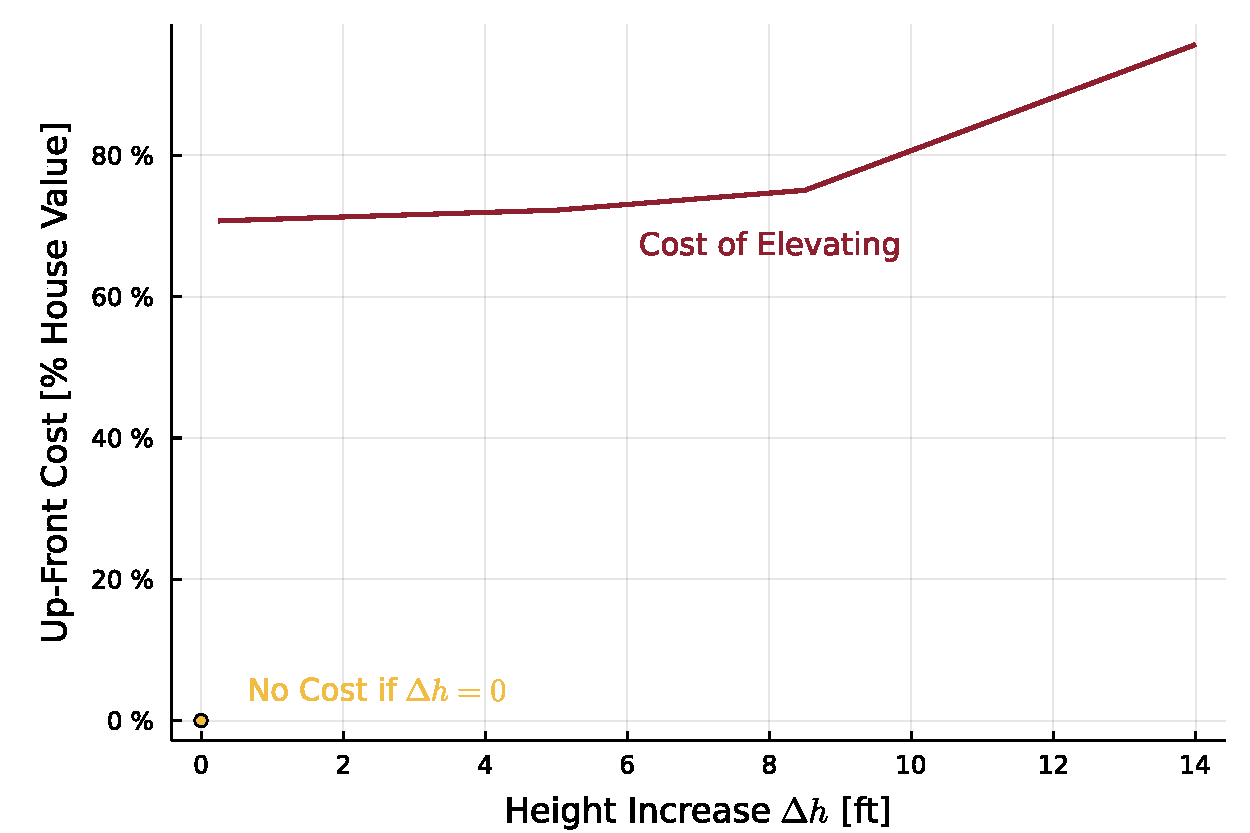
\includegraphics[width=4in]{cost-up-front}
    \caption{
        Following \citet{zarekarizi_suboptimal:2020}, we model the cost of elevating a single-family house by interpolating estimates from the Coastal Louisiana Risk Assessment Model \citep{johnson_clara:2013}.
        According to this model, the unit cost of elevating a house by 3-7, 7-10, and 10-14 feet is \usd{82.50}, \usd{86.25}, and \usd{103.75} per square foot, respectively, with a \usd{20745} initial cost.
        Values are sensitive to house floor area and structural value; see \cref{tab:uncertainties}.
    }\label{fig:cost-up-front}
\end{figure}

\begin{figure}
    \centering
    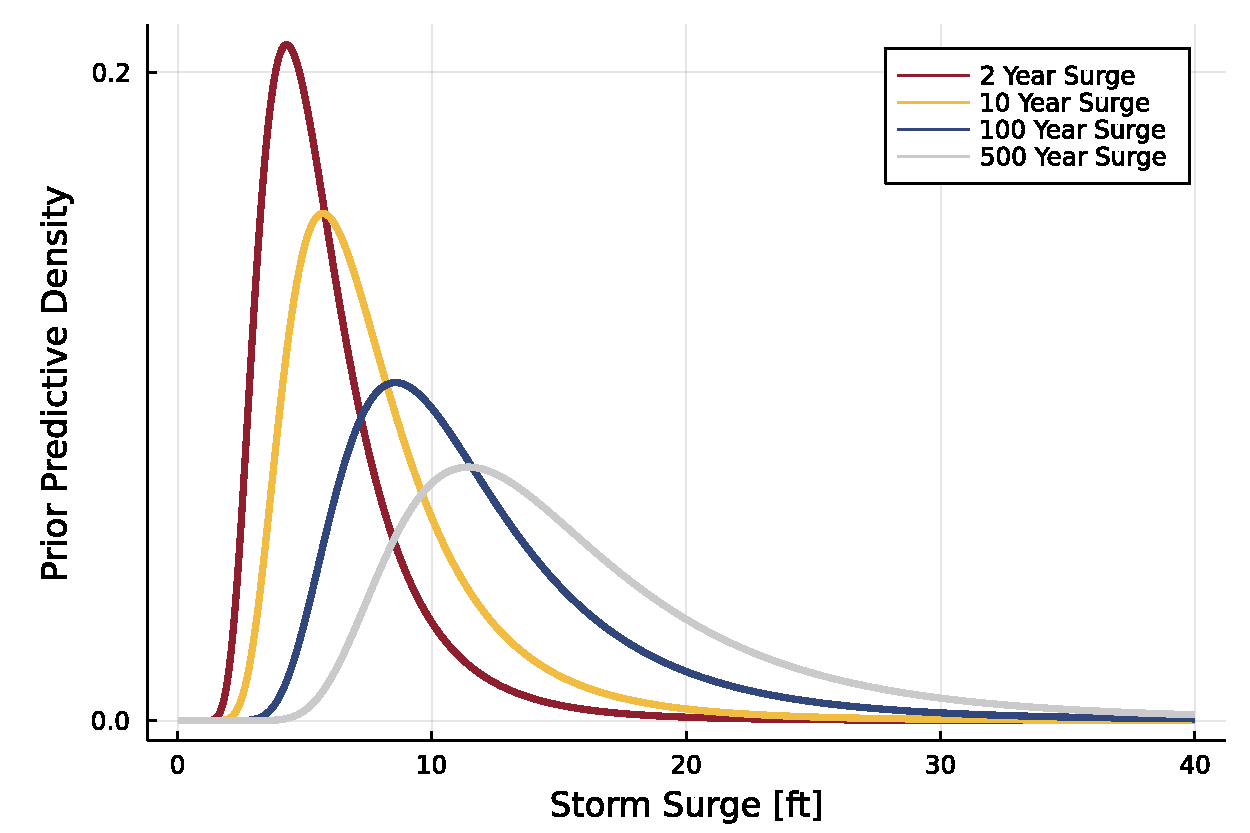
\includegraphics[width=4in]{surge-gev-priors}
    \caption{
        Prior distributions for annual maximum storm surge.
        Rather than apply a prior over model parameters directly, we apply a weakly informative prior over quantiles of the resulting distribution (that is, over a function of the model parameters) following \citet{coles_evd:1996}.
        See \cref{sec:storm-surge} for details.
        For the 2, 10, 100, and 500 year events we apply Normal distributions, truncated at zero, with means \SIlist{4;6;10;15}{ft} and standard deviations \SIlist{1.5;1.75;2.25;2.75}{ft}, respectively.
    }\label{fig:surge-gev-priors}
\end{figure}

\begin{figure}
    \centering
    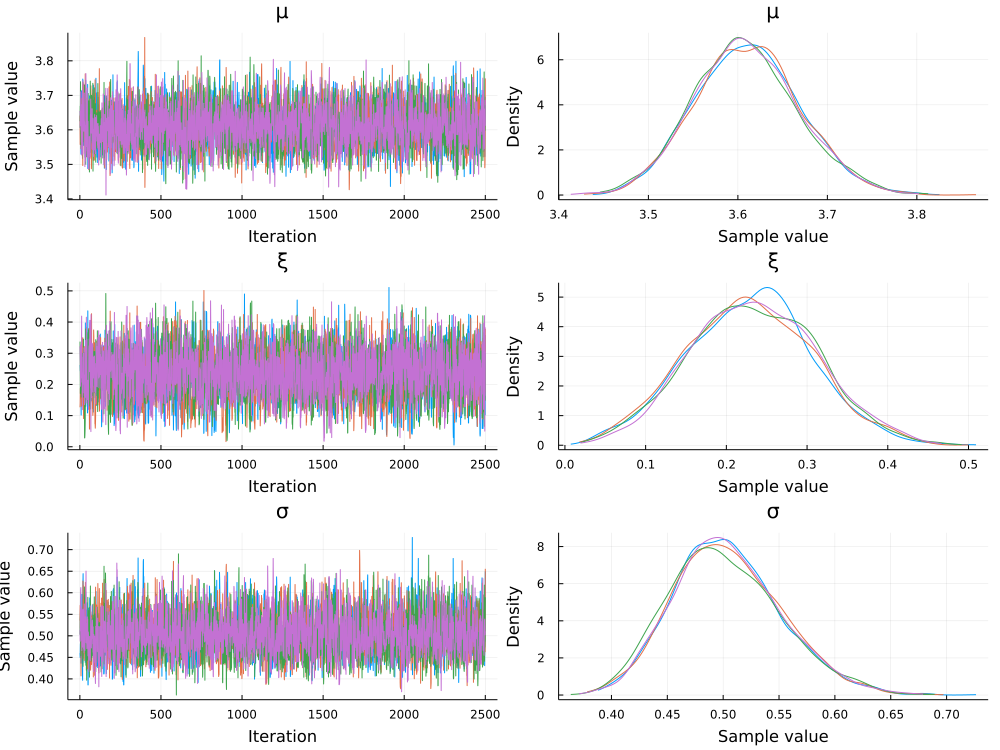
\includegraphics[width=\textwidth]{surge-posterior-chains}
    \caption{
        \Gls{mcmc} plots for posterior draws from the storm surge model.
        We draw \num{10000} samples by running four chains of \num{3500} iterations each and discarding the first \num{1000}.
        The mixing of the chains is consistent with, though does not guarantee, convergence.
    }\label{fig:surge-posterior-chains}
\end{figure}

\begin{figure}
    \centering
    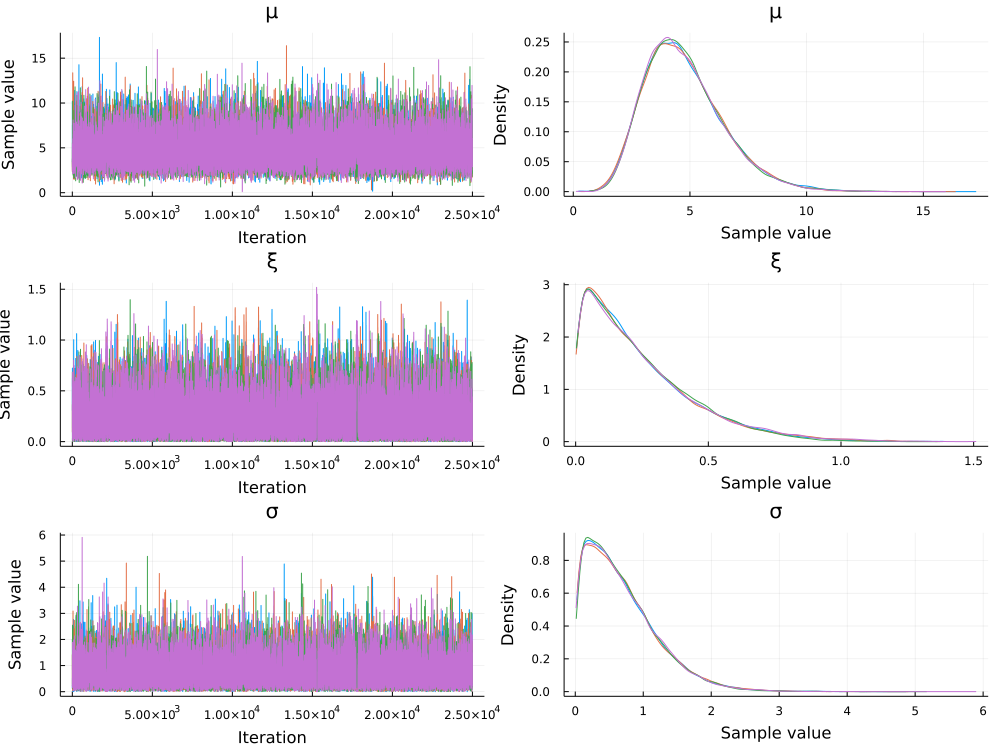
\includegraphics[width=\textwidth]{surge-prior-chains}
    \caption{
        As \cref{fig:surge-posterior-chains} but for draws from the prior distribution.
    }\label{fig:surge-prior-chains}
\end{figure}

\begin{figure}
    \centering
    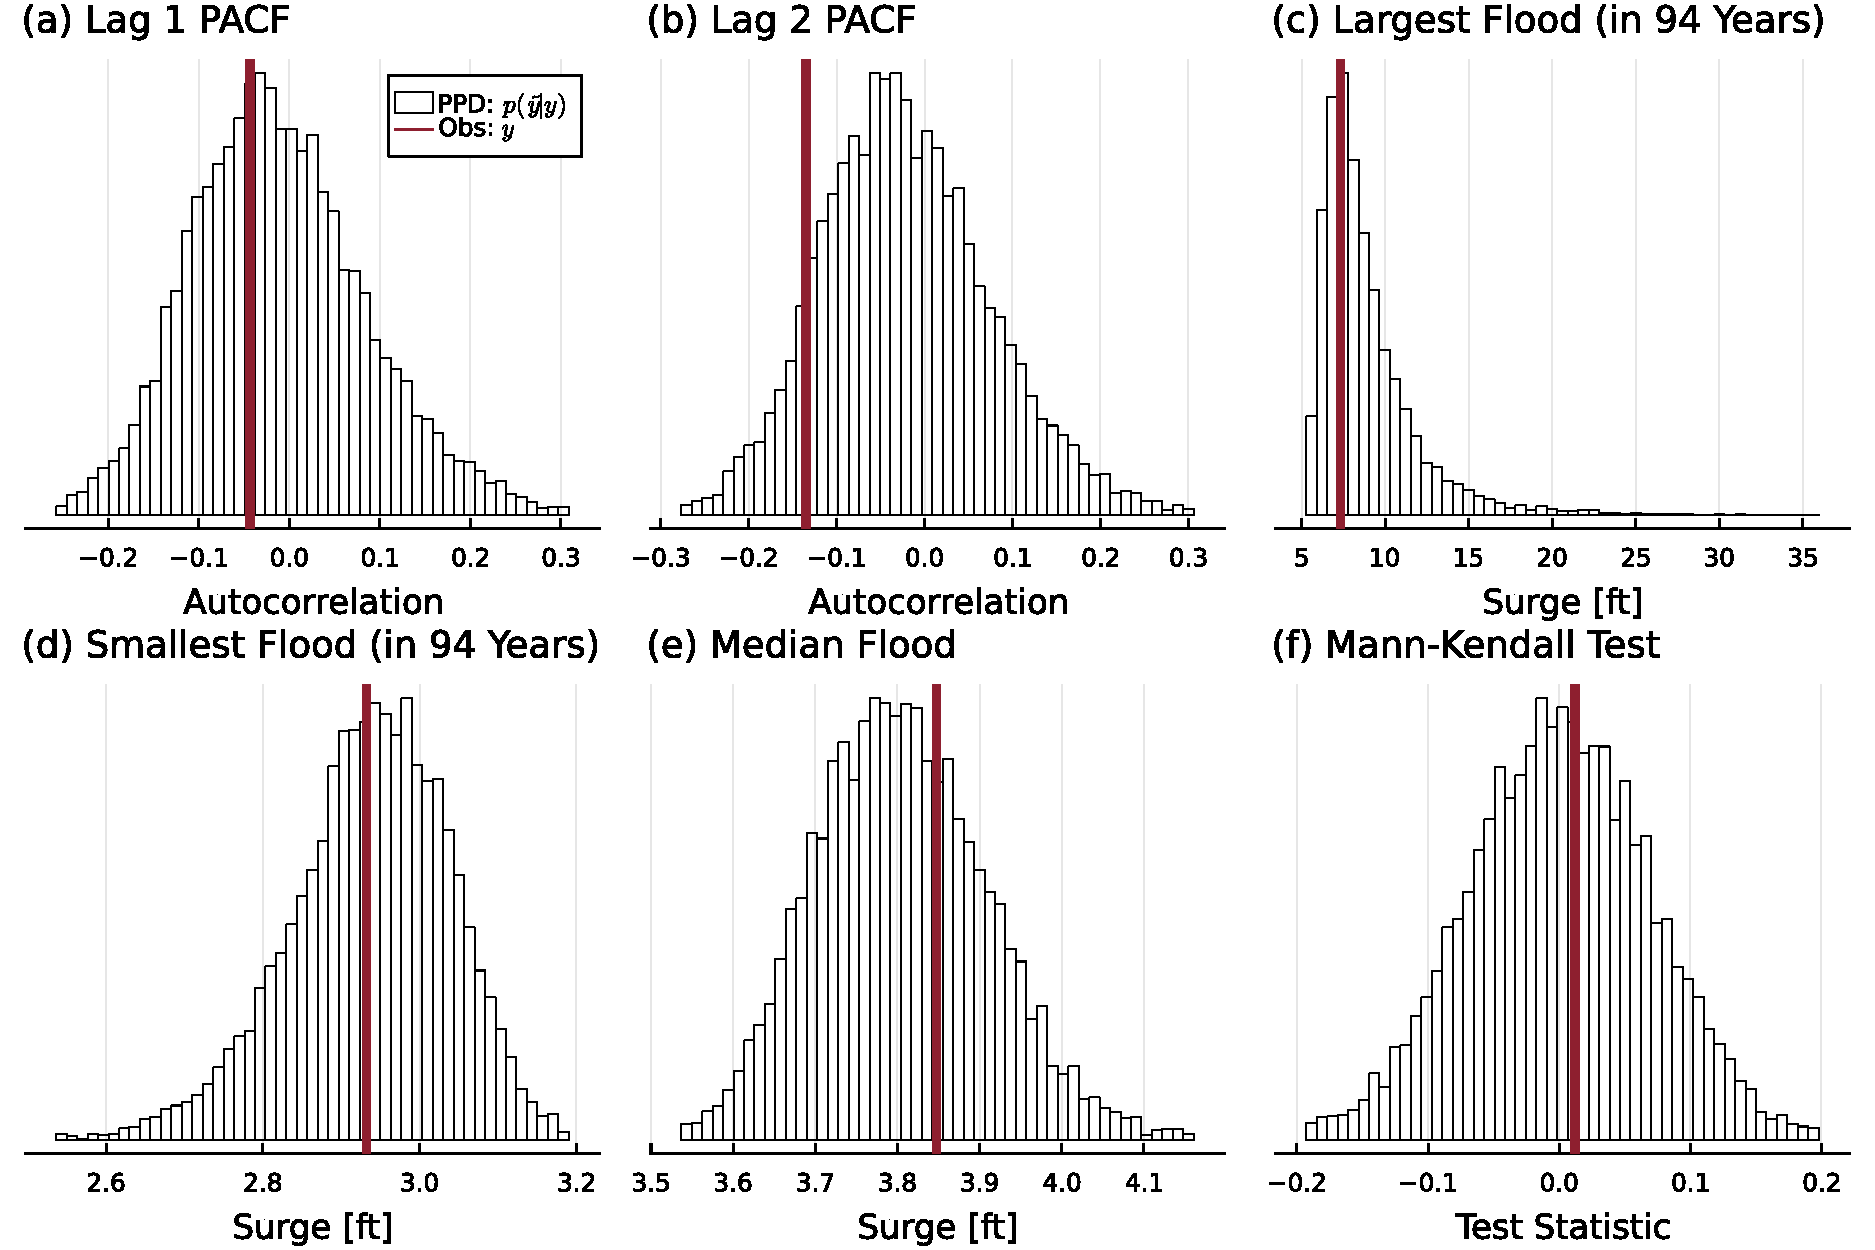
\includegraphics[width=\textwidth]{surge-test-statistics}
    \caption{
        Posterior predictive checks for the stationary \gls{gev} storm surge model (\cref{sec:storm-surge}).
        Each panel shows a different test statistic: partial autocorrelation at lags 1 and 2; sample maximum; sample minimum; sample median; and Mann-Kendall trend test statistic.
        The histograms show the distribution of each test statistic from the posterior predictive distribution.
        Orange lines show the test statistic's value in the observed data.
        Observed values near the mode of the posterior predictive distribution are consistent with, but do not guarantee, a good fit.
        For further discussion of posterior predictive checks, see Chapter 6 of \citet{Gelman:2014tc}.
    }\label{fig:surge-test-statistics}
\end{figure}

\begin{figure}
    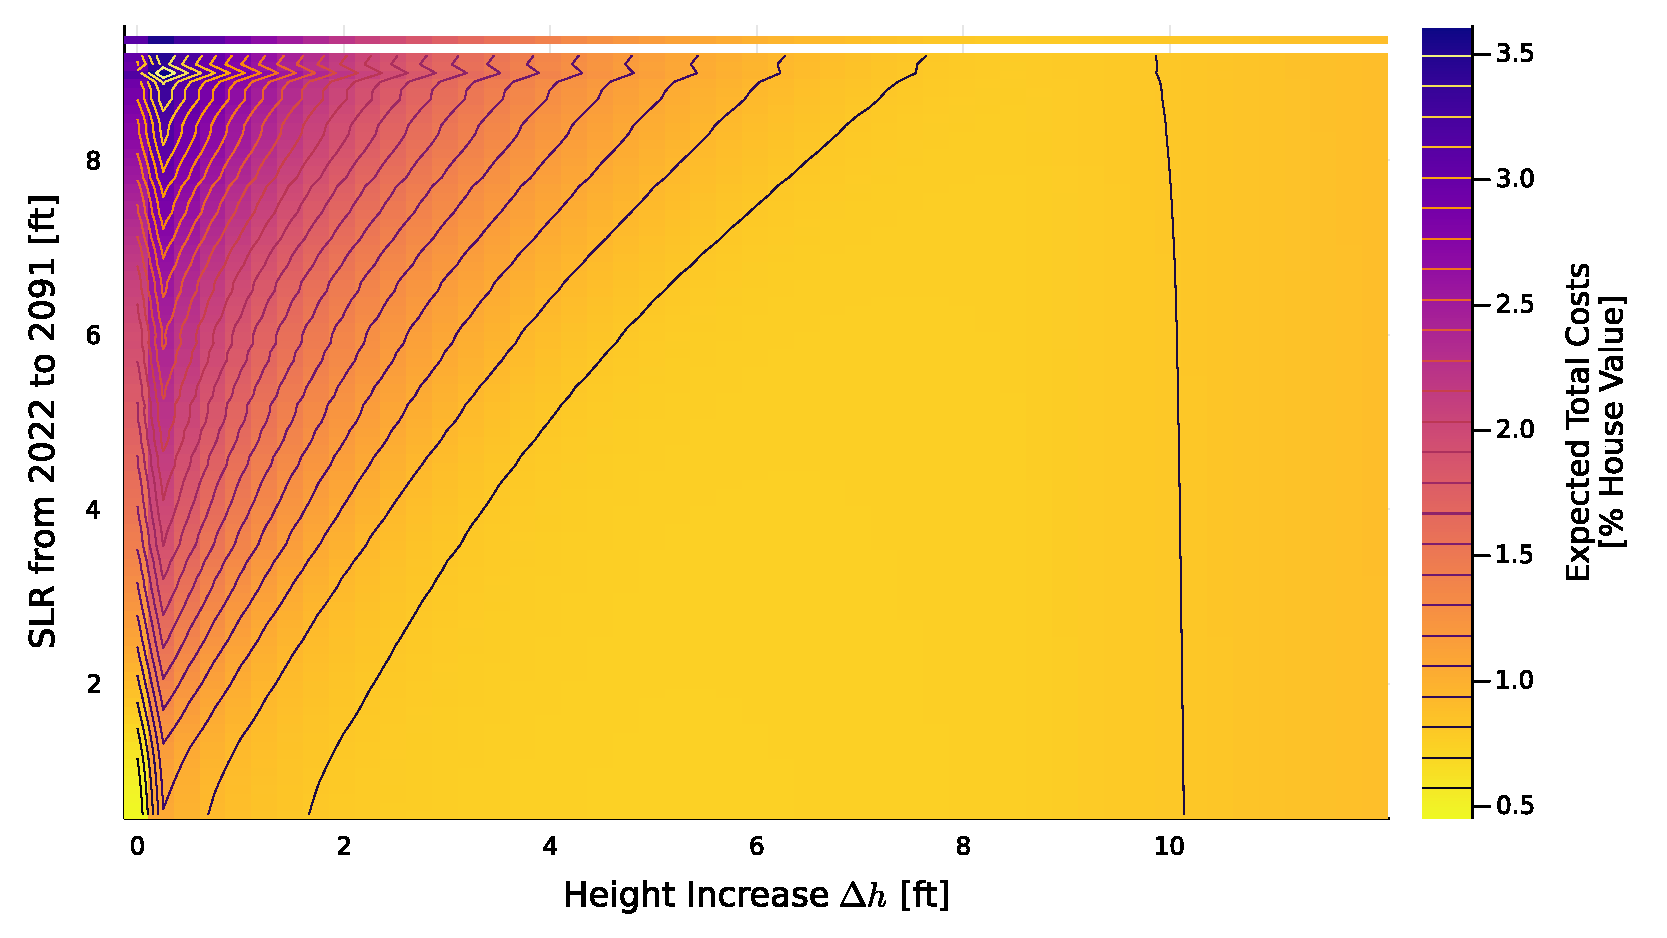
\includegraphics[width=\textwidth]{scenario-map-height-slr}
    \caption{
        Expected total lifetime cost (damages plus up-front cost) as a function of sea level rise over the house lifetime and height increase $\Delta h$.
        Initial house elevation is fixed to \SI{1}{ft} below the \gls{bfe}.
    }\label{fig:scenario-map-height-slr}
\end{figure}

\section{Supplemental tables}

\begin{table}[h]
    \centering
    \caption{
        Diagnostic statistics for the \gls{mcmc} sampling for the storm surge posterior draws.
        Statistics include the mean and standard deviation of each parameter, the naive standard error and Monte Carlo standard error (which measure uncertainty in the mean), the effective sample size, $\hat{R}$ diagnostic, and effective samples per second, which describes sampling speed.
        In general, a $\hat{R}$ value close to one is consistent with, though does not guarantee, convergence.
    }\label{tab:surge-posterior-mcmc-diagnostics}
    \begin{tabular}{cccccccc}
\toprule
$\textrm{Parameter}$ & $\textrm{Mean}$ & $\textrm{Stdev.}$ & $\textrm{Naive SE}$ & $\textrm{MCSE}$ & $\textrm{ESS}$ & $\hat{R}$ & $ess_{per\_sec}$\\
\midrule
$\mu$ & $3.610$ & $0.058$ & $0.001$ & $0.001$ & $4819.426$ & $1.000$ & $467.044$\\
$\sigma$ & $0.504$ & $0.049$ & $0.000$ & $0.001$ & $4508.859$ & $1.000$ & $436.947$\\
$\xi$ & $0.231$ & $0.078$ & $0.001$ & $0.001$ & $4729.255$ & $1.001$ & $458.306$\\
\bottomrule
\end{tabular}

\end{table}

\begin{table}[h]
    \centering
    \caption{As \cref{tab:surge-posterior-mcmc-diagnostics} but for draws from the prior distribution.}\label{tab:surge-prior-mcmc-diagnostics}
    \begin{tabular}{ccccccc}
\toprule
$\textrm{Parameter}$ & $\textrm{Mean}$ & $\textrm{Stdev.}$ & $\textrm{Naive SE}$ & $\textrm{MCSE}$ & $\textrm{ESS}$ & $\hat{R}$\\
\midrule
$\mu$ & $4.774$ & $1.702$ & $0.005$ & $0.011$ & $26657.405$ & $1.000$\\
$\xi$ & $0.246$ & $0.215$ & $0.001$ & $0.002$ & $11238.145$ & $1.000$\\
$\sigma$ & $0.682$ & $0.531$ & $0.002$ & $0.004$ & $24720.263$ & $1.000$\\
\bottomrule
\end{tabular}

\end{table}

\end{document}
